% *** Authors should verify (and, if needed, correct) their LaTeX system  ***
% *** with the testflow diagnostic prior to trusting their LaTeX platform ***
% *** with production work. IEEE's font choices can trigger bugs that do  ***
% *** not appear when using other class files.                            ***
% The testflow support page is at:
% http://www.michaelshell.org/tex/testflow/


%%*************************************************************************
%% Legal Notice:
%% This code is offered as-is without any warranty either expressed or
%% implied; without even the implied warranty of MERCHANTABILITY or
%% FITNESS FOR A PARTICULAR PURPOSE!
%% User assumes all risk.
%% In no event shall IEEE or any contributor to this code be liable for
%% any damages or losses, including, but not limited to, incidental,
%% consequential, or any other damages, resulting from the use or misuse
%% of any information contained here.
%%
%% All comments are the opinions of their respective authors and are not
%% necessarily endorsed by the IEEE.
%%
%% This work is distributed under the LaTeX Project Public License (LPPL)
%% ( http://www.latex-project.org/ ) version 1.3, and may be freely used,
%% distributed and modified. A copy of the LPPL, version 1.3, is included
%% in the base LaTeX documentation of all distributions of LaTeX released
%% 2003/12/01 or later.
%% Retain all contribution notices and credits.
%% ** Modified files should be clearly indicated as such, including  **
%% ** renaming them and changing author support contact information. **
%%
%% File list of work: IEEEtran.cls, New_IEEEtran_how-to.pdf, bare_jrnl_new_sample4.tex,
%%*************************************************************************
\PassOptionsToPackage{unicode}{hyperref}
\PassOptionsToPackage{hyphens}{url}
\PassOptionsToPackage{dvipsnames,svgnames,x11names}{xcolor}
% Note that the a4paper option is mainly intended so that authors in
% countries using A4 can easily print to A4 and see how their papers will
% look in print - the typesetting of the document will not typically be
% affected with changes in paper size (but the bottom and side margins will).
% Use the testflow package mentioned above to verify correct handling of
% both paper sizes by the user's LaTeX system.
%
% Also note that the "draftcls" or "draftclsnofoot", not "draft", option
% should be used if it is desired that the figures are to be displayed in
% draft mode.
%
\documentclass[
  journal,
]{IEEEtran}%
% If IEEEtran.cls has not been installed into the LaTeX system files,
% manually specify the path to it like:
% \documentclass[journal]{../sty/IEEEtran}
\usepackage[cmex10]{amsmath}
\usepackage{amssymb}
\usepackage{iftex}
\ifPDFTeX
  \usepackage[T1]{fontenc}
  \usepackage[utf8]{inputenc}
  \usepackage{textcomp} % provide euro and other symbols
\else % if luatex or xetex
  \usepackage{unicode-math} % this also loads fontspec
  \defaultfontfeatures{Scale=MatchLowercase}
  \defaultfontfeatures[\rmfamily]{Ligatures=TeX,Scale=1}
\fi
%\usepackage{lmodern}
\ifPDFTeX\else
\fi
% Use upquote if available, for straight quotes in verbatim environments
\IfFileExists{upquote.sty}{\usepackage{upquote}}{}
\IfFileExists{microtype.sty}{% use microtype if available
  \usepackage[]{microtype}
  \UseMicrotypeSet[protrusion]{basicmath} % disable protrusion for tt fonts
}{}
\makeatletter
\parindent    1.0em
\ifCLASSOPTIONcompsoc
  \parindent    1.5em
\fi
\makeatother
\usepackage{xcolor}
\setlength{\emergencystretch}{3em} % prevent overfull lines

\setcounter{secnumdepth}{5}
% Make \paragraph and \subparagraph free-standing
\ifx\paragraph\undefined\else
  \let\oldparagraph\paragraph
  \renewcommand{\paragraph}[1]{\oldparagraph{#1}\mbox{}}
\fi
\ifx\subparagraph\undefined\else
  \let\oldsubparagraph\subparagraph
  \renewcommand{\subparagraph}[1]{\oldsubparagraph{#1}\mbox{}}
\fi


\providecommand{\tightlist}{%
  \setlength{\itemsep}{0pt}\setlength{\parskip}{0pt}}\usepackage{longtable,booktabs,array}
\usepackage{calc} % for calculating minipage widths
% Correct order of tables after \paragraph or \subparagraph
\usepackage{etoolbox}
\makeatletter
\patchcmd\longtable{\par}{\if@noskipsec\mbox{}\fi\par}{}{}
\makeatother
% Allow footnotes in longtable head/foot
\IfFileExists{footnotehyper.sty}{\usepackage{footnotehyper}}{\usepackage{footnote}}
\makesavenoteenv{longtable}
\usepackage{graphicx}
\makeatletter
\def\maxwidth{\ifdim\Gin@nat@width>\linewidth\linewidth\else\Gin@nat@width\fi}
\def\maxheight{\ifdim\Gin@nat@height>\textheight\textheight\else\Gin@nat@height\fi}
\makeatother
% Scale images if necessary, so that they will not overflow the page
% margins by default, and it is still possible to overwrite the defaults
% using explicit options in \includegraphics[width, height, ...]{}
\setkeys{Gin}{width=\maxwidth,height=\maxheight,keepaspectratio}
% Set default figure placement to htbp
\makeatletter
\def\fps@figure{htbp}
\makeatother
\newlength{\cslhangindent}
\setlength{\cslhangindent}{1.5em}
\newlength{\csllabelwidth}
\setlength{\csllabelwidth}{3em}
\newlength{\cslentryspacingunit} % times entry-spacing
\setlength{\cslentryspacingunit}{\parskip}
\newenvironment{CSLReferences}[2] % #1 hanging-ident, #2 entry spacing
 {% don't indent paragraphs
  \setlength{\parindent}{0pt}
  % turn on hanging indent if param 1 is 1
  \ifodd #1
  \let\oldpar\par
  \def\par{\hangindent=\cslhangindent\oldpar}
  \fi
  % set entry spacing
  \setlength{\parskip}{#2\cslentryspacingunit}
 }%
 {}
\usepackage{calc}
\newcommand{\CSLBlock}[1]{#1\hfill\break}
\newcommand{\CSLLeftMargin}[1]{\parbox[t]{\csllabelwidth}{#1}}
\newcommand{\CSLRightInline}[1]{\parbox[t]{\linewidth - \csllabelwidth}{#1}\break}
\newcommand{\CSLIndent}[1]{\hspace{\cslhangindent}#1}

\usepackage{physics}
\usepackage[version=3]{mhchem}
\usepackage{orcidlink}
\usepackage{float}
\floatplacement{table}{htb}
\makeatletter
\makeatother
\makeatletter
\makeatother
\makeatletter
\@ifpackageloaded{caption}{}{\usepackage{caption}}
\AtBeginDocument{%
\ifdefined\contentsname
  \renewcommand*\contentsname{Table of contents}
\else
  \newcommand\contentsname{Table of contents}
\fi
\ifdefined\listfigurename
  \renewcommand*\listfigurename{List of Figures}
\else
  \newcommand\listfigurename{List of Figures}
\fi
\ifdefined\listtablename
  \renewcommand*\listtablename{List of Tables}
\else
  \newcommand\listtablename{List of Tables}
\fi
\ifdefined\figurename
  \renewcommand*\figurename{Fig.}
\else
  \newcommand\figurename{Fig.}
\fi
\ifdefined\tablename
  \renewcommand*\tablename{Table}
\else
  \newcommand\tablename{Table}
\fi
}
\@ifpackageloaded{float}{}{\usepackage{float}}
\floatstyle{ruled}
\@ifundefined{c@chapter}{\newfloat{codelisting}{h}{lop}}{\newfloat{codelisting}{h}{lop}[chapter]}
\floatname{codelisting}{Listing}
\newcommand*\listoflistings{\listof{codelisting}{List of Listings}}
\makeatother
\makeatletter
\@ifpackageloaded{caption}{}{\usepackage{caption}}
\@ifpackageloaded{subcaption}{}{\usepackage{subcaption}}
\makeatother
\makeatletter
\@ifpackageloaded{tcolorbox}{}{\usepackage[skins,breakable]{tcolorbox}}
\makeatother
\makeatletter
\@ifundefined{shadecolor}{\definecolor{shadecolor}{rgb}{.97, .97, .97}}
\makeatother
\makeatletter
\makeatother
\makeatletter
\makeatother
\usepackage[skip=2pt,font=footnotesize]{caption}
%\captionsetup{format=myformat}
\makeatletter
%\setlength{\cslhangindent}{0pt plus .5pt}
\providecommand{\bibfont}{\footnotesize}
\let\CSLReferences@rig=\CSLReferences
\renewcommand{\CSLReferences}[2]{
\bibfont\settowidth\csllabelwidth{[999]}
\CSLReferences@rig{#1}{#2}
\vskip 0.3\baselineskip plus 0.1\baselineskip minus 0.1\baselineskip%
}
\makeatother
\ifLuaTeX
  \usepackage{selnolig}  % disable illegal ligatures
\fi
\IfFileExists{bookmark.sty}{\usepackage{bookmark}}{\usepackage{hyperref}}
\IfFileExists{xurl.sty}{\usepackage{xurl}}{} % add URL line breaks if available
\urlstyle{same} % disable monospaced font for URLs
\hypersetup{
  pdftitle={Optimierung der Preisstrategien bei Airbnb: Eine Analyse zur Maximierung der Einnahmen},
  pdfauthor={Cedric Gisler \& Jovan Pajic},
  colorlinks=true,
  linkcolor={blue},
  filecolor={Maroon},
  citecolor={Blue},
  urlcolor={Blue},
  pdfcreator={LaTeX via pandoc}}

% *** Do not adjust lengths that control margins, column widths, etc. ***
% *** Do not use packages that alter fonts (such as pslatex).         ***
% There should be no need to do such things with IEEEtran.cls V1.6 and later.
% (Unless specifically asked to do so by the journal or conference you plan
% to submit to, of course. )


% correct bad hyphenation here
\hyphenation{op-tical net-works semi-conduc-tor}

%
% paper title
% can use linebreaks \\ within to get better formatting as desired
% Do not put math or special symbols in the title.
% paper title
% can use linebreaks \\ within to get better formatting as desired
% Do not put math or special symbols in the title.
\title{Optimierung der Preisstrategien bei Airbnb: Eine Analyse zur
Maximierung der Einnahmen}

\author{
Cedric Gisler \& Jovan Pajic%

}
\begin{document}

% The paper headers

% use for special paper notices

% make the title area
\maketitle

% As a general rule, do not put math, special symbols or citations
% in the abstract or keywords.
% Note that keywords are not normally used for peerreview papers.

% For peer review papers, you can put extra information on the cover
% page as needed:
% \ifCLASSOPTIONpeerreview
% \begin{center} \bfseries EDICS Category: 3-BBND \end{center}
% \fi
%
% For peerreview papers, this IEEEtran command inserts a page break and
% creates the second title. It will be ignored for other modes.
% \IEEEpeerreviewmaketitle

\ifdefined\Shaded\renewenvironment{Shaded}{\begin{tcolorbox}[interior hidden, borderline west={3pt}{0pt}{shadecolor}, breakable, enhanced, sharp corners, frame hidden, boxrule=0pt]}{\end{tcolorbox}}\fi

\hypertarget{abstrakt}{%
\section{Abstrakt}\label{abstrakt}}

In der heutigen dynamischen Welt des Online-Tourismus ist Airbnb eine
zentrale Plattform für die Buchung von Unterkünften. Diese Arbeit
untersucht die Faktoren, die den Preis pro Person einer
Airbnb-Unterkunft beeinflussen, um Gastgebern datenbasierte Empfehlungen
zur Optimierung ihrer Preisstrategien zu geben. Mithilfe von
deskriptiver Statistik, Korrelationsanalysen und linearen
Regressionsmodellen analysieren wir die Daten von Airbnb-Unterkünften in
Zürich, Vaud und Genf. Die Ergebnisse zeigen, dass die
Sauberkeitsbewertung der Unterkünfte, die Anzahl der Listings eines
Hosts sowie die Verfügbarkeit wesentliche Einflussfaktoren sind.
Basierend auf diesen Erkenntnissen entwickeln wir prädiktive Modelle zur
Vorhersage des Preises pro Person. Unsere Analyse bietet Einblicke für
Gastgeber, die ihre Preisstrategien verbessern und ihre Einnahmen
maximieren möchten.

\hypertarget{einleitung-mit-forschungsfrage-d.h.-geschuxe4ftsfrage-am-ende}{%
\section{Einleitung (mit Forschungsfrage (d.h. Geschäftsfrage) am
Ende)}\label{einleitung-mit-forschungsfrage-d.h.-geschuxe4ftsfrage-am-ende}}

In der heutigen, schnelllebigen Welt des Online-Tourismus spielen
Plattformen wie Airbnb eine zentrale Rolle bei der Art und Weise, wie
Menschen reisen und Unterkünfte buchen. Airbnb bietet eine Vielzahl von
Unterkünften an, von einfachen Zimmern bis hin zu luxuriösen Villen. So
vielfältig wie das Angebot sind auch die Vorlieben und Erwartungen der
Gäste. Vor diesem Hintergrund stellt sich die Forschungsfrage:
\textbf{\emph{Welche Eigenschaften einer Airbnb-Unterkunft ziehen Gäste
an und ermöglichen es, einen höheren Preis pro Apparment zu erzielen?}}

Der grösste Unterschied eines Airbnbs ist deren Grösse. Eine der
wichtigsten Eigenschaften eines Apartments ist aber die Lage, die
Bewertung und der Gastgeber, somit definieren wir folgende
Nullhypothesen:

\begin{enumerate}
\def\labelenumi{\arabic{enumi}.}
\item
  \textbf{Bewertung der Airbnb-Unterkünften:}

  \begin{itemize}
  \tightlist
  \item
    \textbf{Nullhypothese (H0):} Die Höhe der Gesamtbewertung
    (review\_scores\_rating) hat keinen signifikanten Einfluss auf den
    Preis pro Person der Unterkunft.
  \item
    \textbf{Alternativhypothese (H1):} Die Höhe der Gesamtbewertung
    (review\_scores\_rating) hat einen signifikanten Einfluss auf den
    Preis pro Person der Unterkunft.
  \item
    \textbf{Fragen:}

    \begin{itemize}
    \tightlist
    \item
      Hat die Gesamtbewertung der Unterkunft (review\_scores\_rating)
      einen signifikanten Einfluss auf den Preis pro Person?
    \item
      Gibt es bestimmte Bewertungsmetriken (z.B. Sauberkeit,
      Kommunikation), die den Preis pro Person stärker beeinflussen als
      andere?
    \end{itemize}
  \end{itemize}
\item
  \textbf{Gastgeber der Airbnb-Unterkunft:}

  \begin{itemize}
  \tightlist
  \item
    \textbf{Nullhypothese (H0):} Die Attribute des Hosts wie
    ``host\_is\_superhost'', ``host\_identity\_verified'' und
    ``host\_listings\_count'' haben keinen signifikanten Einfluss auf
    den Preis pro Person der Unterkunft.
  \item
    \textbf{Alternativhypothese (H1):} Die Attribute des Hosts wie
    ``host\_is\_superhost'', ``host\_identity\_verified'' und
    ``host\_listings\_count'' haben einen signifikanten Einfluss auf den
    Preis pro Person der Unterkunft.
  \item
    \textbf{Fragen:}

    \begin{itemize}
    \item
      Beeinflusst der Status ``Superhost'' (host\_is\_superhost) den
      Preis pro Person?
    \item
      Hat die Verifizierung des Hosts (host\_identity\_verified) einen
      Einfluss auf den Preis pro Person?
    \item
      Wie beeinflusst die Anzahl der Listings eines Hosts
      (host\_listings\_count) den Preis pro Person?
    \end{itemize}
  \end{itemize}
\item
  \textbf{Lage des Airbnb:}

  \begin{itemize}
  \item
    \textbf{Nullhypothese (H0):} Die Entfernung zum Stadtzentrum
    (berechnet durch geografische Koordinaten) hat keinen signifikanten
    Einfluss auf den Preis pro Person der Unterkunft.
  \item
    \textbf{Alternativhypothese (H1):} Die Entfernung zum Stadtzentrum
    (berechnet durch geografische Koordinaten) hat einen signifikanten
    Einfluss auf den Preis pro Person der Unterkunft.
  \item
    \textbf{Fragen:}

    \begin{itemize}
    \tightlist
    \item
      Beeinflusst die Entfernung zum Stadtzentrum den Preis pro Person
      der Unterkunft?
    \item
      Gibt es andere geografische Faktoren (z.B. Nähe zu bestimmten
      Attraktionen), die den Preis pro Person beeinflussen?
    \end{itemize}
  \end{itemize}
\end{enumerate}

Weitere wichtige Eigenschaften sind Ereignisse (z.B. Zürich:
Streetparade, Zürich Film Festival) in der betreffenden Stadt. Da wir
aber die Daten nur zu einem einzelnen Zeitpunkt haben und keine
Zeitserie, können wir den Einfluss dieser Ereignisse auf den Preis pro
Person der Unterkunft nicht untersuchen.

\textbf{Deskriptive Analyse:} Wir möchten überprüfen, ob unsere
Hypothesen so stimmen und wir mit unserer Annahme über die Einflüsse auf
den Preis pro Person der Unterkunft richtig liegen.

\textbf{Prädiktive Analyse:} Wir möchten den Trend des Preises pro
Person der Unterkunft aufzeigen und untersuchen, ob wir mithilfe der
Bewertung und den wichtigsten Eigenschaften einer Unterkunft eine
Prognose über den Preis machen können.

\textbf{Präskriptive Analyse:} Wir möchten zeigen, welche Eigenschaften
wie verbessert werden müssen, um die Preise pro Person der Unterkunft
signifikant erhöhen zu können, um einen höheren Preis erzielen zu
können.

\#Datenquelle (mit Angaben zu Quelle, Qualität und Bereinigungsschritten
der Daten)

Die Daten für diese Analyse stammen von der Inside Airbnb Organisation
\protect\hyperlink{ref-inside-airbnb-2023}{{[}1{]}}, die sich dafür
einsetzt, ihre Gemeinden vor den negativen Auswirkungen von
Kurzzeitvermietungen zu schützen. Diese Organisation sammelt und
veröffentlicht regelmässig aktualisierte Datensätze, die aus öffentlich
verfügbaren Informationen auf der Airbnb-Website stammen. Diese
Datensätze würden wir als Vertrauenswürdig einstufen.

Die extrahierten Datensätze umfassen Informationen aus drei bedeutenden
Regionen in der Schweiz: Zürich (27. Dezember 2023), Genénve (27.
Dezember 2023) und Vaud (10. März 2024).

Die Daten umfassen verschiedene Dateien für jede Stadt, wobei für die
Analyse hauptsächlich das ``listings\_long.csv''-File verwendet wird, da
es für die Geschäftsfragen relevant ist. Die Qualität der Daten in
diesem File ist insgesamt sehr hoch, mit wenigen leeren Feldern und
einer konsistenten Struktur innerhalb der Spalten.

Es werden insgesamt 3 Datensätze verwendet, die dieselbe Struktur
aufweisen, jedoch aus drei verschiedenen Regionen stammen, die wir hier
analysieren möchten.

Einige Spalten, wie ``description'', ``neighborhood\_overview'',
``host\_neighborhood'', ``neighborhood'', und die Beschreibung der
Liegenschaft, wie ``bathrooms'' und ``bedrooms'', weisen eine
beträchtliche Anzahl leerer Felder auf. Es wird vermutet, dass diese
Felder optional für die Gastgeber sind und daher nicht immer ausgefüllt
werden. Ebenso fehlt bei einigen Einträgen der Preis, was eine Analyse
erfordert, um mögliche Korrelationen mit anderen Feldern, wie dem ersten
Review, zu identifizieren.

Trotz dieser kleinen Unregelmässigkeiten ist die Datenqualität insgesamt
hoch, und die Beschreibung der Datenfelder wird durch das Data
Dictionary \protect\hyperlink{ref-inside-airbnb-2022}{{[}2{]}} gut
unterstützt.

\textbf{Datenbereinigungsschritte:}

\begin{enumerate}
\def\labelenumi{\arabic{enumi}.}
\item
  \textbf{Entfernung irrelevanter oder leerer Spalten:} Vor der Analyse
  wurden alle Spalten entfernt, die für die Fragestellungen nicht
  relevant sind oder leere Felder enthalten.
\item
  \textbf{Überprüfung der Einheitlichkeit und Konsistenz der Werte:} Die
  verbleibenden Spalten wurden auf Einheitlichkeit der Werte und
  Konsistenz der ``N/A''-Kennzeichnungen überprüft, um sicherzustellen,
  dass die Daten konsistent und interpretierbar sind.
\item
  \textbf{Analyse von Einträgen ohne Preisangabe:} Einige Einträge
  weisen keine Preisangabe auf, was eine Analyse erfordert, um mögliche
  Korrelationen mit anderen Feldern, wie dem ersten Review, zu
  identifizieren. Je nach Ergebnis dieser Analyse könnten Einträge ohne
  Preisangabe entfernt oder anderweitig behandelt werden, um die
  Datenintegrität zu gewährleisten.
\end{enumerate}

\hypertarget{datenqualituxe4t-analyse-im-hinblick-auf-datenqualituxe4tsaspekte}{%
\section{Datenqualität (Analyse im Hinblick auf
Datenqualitätsaspekte)}\label{datenqualituxe4t-analyse-im-hinblick-auf-datenqualituxe4tsaspekte}}

Nachdem wir die Zusammenfassung der Daten betrachtet und eine Analyse
der Datensätze durchgeführt haben, haben wir die folgenden
Datenanpassungen vorgenommen:

\begin{enumerate}
\def\labelenumi{\arabic{enumi}.}
\item
  Konvertiere \textbf{\texttt{host\_response\_rate}} von Zeichenfolge
  (chr) in Ganzzahl (integer), wobei ``N/A'' durch NA ersetzt wird.
  Entferne das Prozentzeichen (\%) und benenne die Spalte in
  \textbf{\texttt{host\_response\_rate\_in\_\%}} um.
\item
  Konvertiere \textbf{\texttt{host\_acceptance\_rate}} von Zeichenfolge
  (chr) in Ganzzahl (integer), wobei ``N/A'' durch NA ersetzt wird.
  Entferne das Prozentzeichen (\%) und benenne die Spalte in
  \textbf{\texttt{host\_acceptance\_rate\_in\_\%}} um.
\item
  Konvertiere \textbf{\texttt{price}} von Zeichenfolge (chr) in
  Dezimalzahl (double), wobei das Dollarzeichen (\$) entfernt wird.
  Benenne die Spalte in \textbf{\texttt{price\_in\_\$}} um.
\item
  Lösche die folgenden Spalten: \textbf{\texttt{description}},
  \textbf{\texttt{neighborhood\_overview}},
  \textbf{\texttt{host\_location}}, \textbf{\texttt{host\_about}},
  \textbf{\texttt{host\_neighbourhood}},
  \textbf{\texttt{host\_verifications}},
  \textbf{\texttt{neighbourhood}},
  \textbf{\texttt{neighbourhood\_cleansed}},
  \textbf{\texttt{bathrooms}}, \textbf{\texttt{bedrooms}},
  \textbf{\texttt{amenities}}, \textbf{\texttt{calendar\_updated}} ,
  \textbf{\texttt{license}}.
\item
  Analysiere fehlende Werte (NA) oder leere Felder und ersetze sie
  gegebenenfalls.
\end{enumerate}

Nach diesen Anpassungen haben wir die Daten weiter analysiert und die
folgenden Schritte durchgeführt:

\begin{enumerate}
\def\labelenumi{\arabic{enumi}.}
\item
  \textbf{Überprüfung auf Duplikate:} Es wurde überprüft, ob es doppelte
  \textbf{\texttt{id}}s in den Daten gibt.
\item
  \textbf{Visualisierung der Verteilungen:} Es wurden Histogramme
  erstellt, um die Verteilungen der Preise, der Bewertungsscores und der
  Bewertungen pro Monat zu visualisieren.
\item
  \textbf{Analyse von Anomalien und Ausreissern:} Da der Preis stark
  variiert, analysieren wir die Möglichkeit, den Preis pro Person zu
  berechnen. Dabei fällt auf, dass der Preis bei ``Entire home/apt'' für
  die maximale Anzahl der Gäste (\textbf{\texttt{accommodates}})
  berechnet wird, was sinnvoll ist, da die gesamte Unterkunft gebucht
  wird. Bei ``Private room'' und ``Shared room'' hingegen wird der Preis
  mehrheitlich pro Person angegeben. Im Gegensatz dazu ist der Preis bei
  ``Hotel room'' wieder für die maximale Gästeanzahl festgelegt.
\item
  \textbf{Export der Datensätze:} Die drei bereinigten Datensätze wurden
  in neuen Dateien erstellt und abgespeichert.
\end{enumerate}

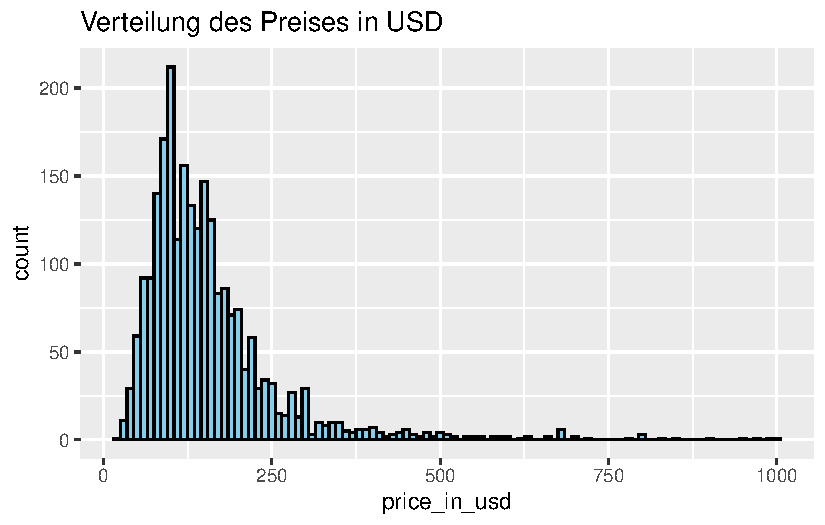
\includegraphics{main_files/figure-pdf/eda-1.pdf}

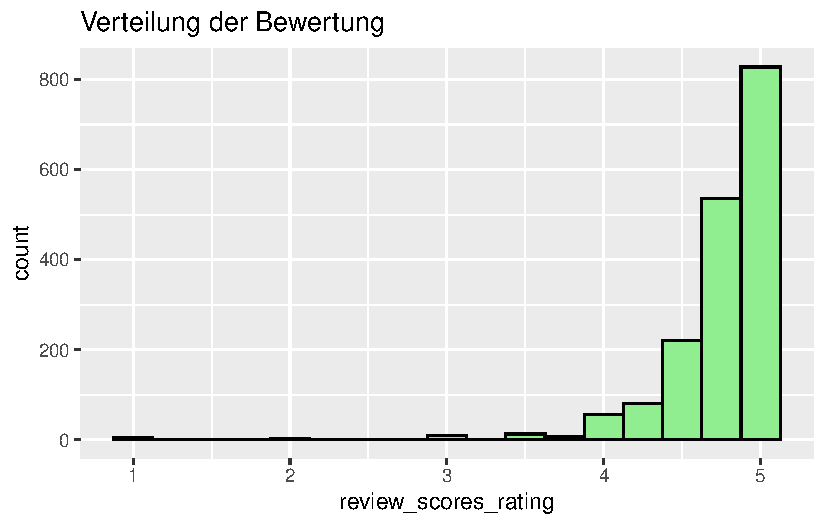
\includegraphics{main_files/figure-pdf/eda-2.pdf}

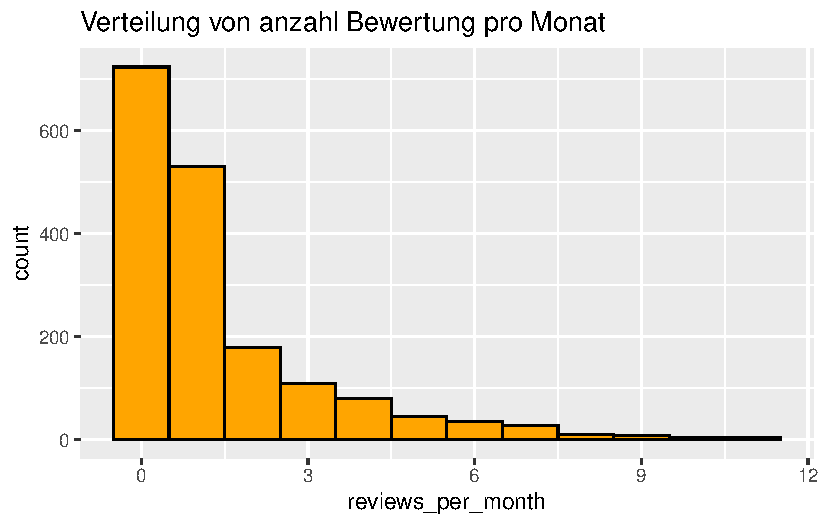
\includegraphics{main_files/figure-pdf/eda-3.pdf}

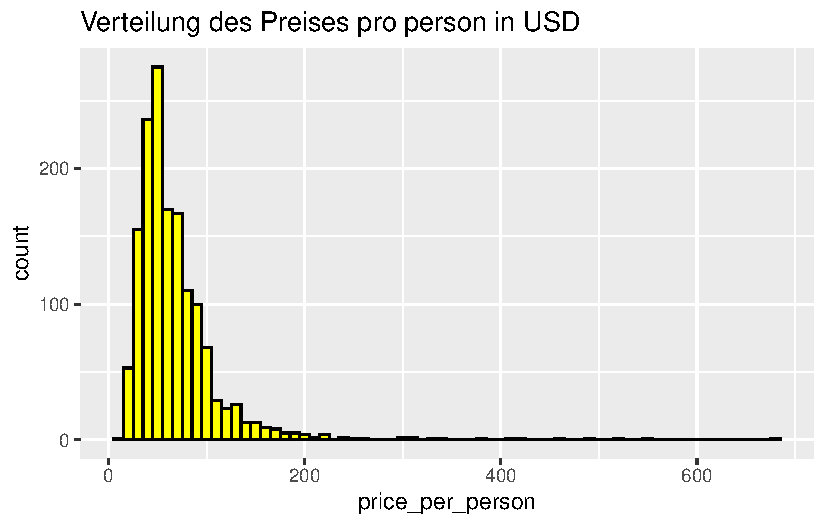
\includegraphics{main_files/figure-pdf/eda price_per_person-1.pdf}

Die analysierten Werte zeigen eine ausgeglichene Verteilung ohne
signifikante Ausreisser oder extreme Werte. Dies deutet darauf hin, dass
der Datenbereinigungsprozess effektiv war und die Daten konsistent und
zuverlässig für weitere Analysen vorliegen.

\hypertarget{datenanalyse-informationen-zur-datenstruktur-organisation-und-zu-den-fuxfcr-die-analyse-verwendeten-methoden}{%
\section{Datenanalyse (Informationen zur Datenstruktur, Organisation und
zu den für die Analyse verwendeten
Methoden)}\label{datenanalyse-informationen-zur-datenstruktur-organisation-und-zu-den-fuxfcr-die-analyse-verwendeten-methoden}}

\hypertarget{datenstruktur-und-organisation}{%
\subsection{Datenstruktur und
Organisation}\label{datenstruktur-und-organisation}}

Die vorliegenden bereinigten Datensets besteht aus Informationen zu
Airbnb-Unterkünften in Zürich, Geneve und Vaud und umfasst 63 Variablen
und mehrere tausend Zeilen, wobei jede Zeile eine einzelne Unterkunft
repräsentiert. Die Variablen enthalten diverse Informationen, darunter:

\begin{itemize}
\item
  \textbf{ID und URLs:} Eindeutige Identifikationsnummern und Links zu
  den Listings.
\item
  \textbf{Host-Informationen:} Daten über die Gastgeber, wie
  \texttt{host\_id}, \texttt{host\_name}, \texttt{host\_is\_superhost},
  \texttt{host\_identity\_verified}, und \texttt{host\_listings\_count}.
\item
  \textbf{Eigenschaften der Unterkunft:} Variablen wie
  \texttt{accommodates}, \texttt{bedrooms}, \texttt{bathrooms},
  \texttt{beds}, \texttt{price\_in\_usd}, und
  \texttt{price\_per\_person}.
\item
  \textbf{Bewertungen:} Bewertungsscores wie
  \texttt{review\_scores\_rating}, \texttt{review\_scores\_cleanliness},
  \texttt{review\_scores\_checkin}, etc.
\item
  \textbf{Geografische Daten:} \texttt{latitude} und \texttt{longitude}.
\item
  \textbf{Verfügbarkeitsdaten:} \texttt{availability\_30},
  \texttt{availability\_60}, \texttt{availability\_90},
  \texttt{availability\_365}.
\end{itemize}

\textbf{Zusammenfassung Preis pro Person und Bewertung Zürich}

\begin{verbatim}
   Min. 1st Qu.  Median    Mean 3rd Qu.    Max. 
  12.75   42.50   56.50   68.79   80.38  676.00 
\end{verbatim}

\begin{verbatim}
   Min. 1st Qu.  Median    Mean 3rd Qu.    Max. 
  1.000   4.660   4.850   4.749   5.000   5.000 
\end{verbatim}

\textbf{Zusammenfassung Preis pro Person und Bewertung Vaud}

\begin{verbatim}
   Min. 1st Qu.  Median    Mean 3rd Qu.    Max. 
   3.75   34.29   47.50   52.96   65.00  310.50 
\end{verbatim}

\begin{verbatim}
   Min. 1st Qu.  Median    Mean 3rd Qu.    Max. 
  1.000   4.670   4.860   4.752   5.000   5.000 
\end{verbatim}

\textbf{Zusammenfassung Preis pro Person und Bewertung Genf}

\begin{verbatim}
   Min. 1st Qu.  Median    Mean 3rd Qu.    Max. 
  13.75   41.50   57.00   64.46   75.50  410.00 
\end{verbatim}

\begin{verbatim}
   Min. 1st Qu.  Median    Mean 3rd Qu.    Max. 
   1.00    4.60    4.82    4.71    5.00    5.00 
\end{verbatim}

\hypertarget{methoden-der-datenanalyse}{%
\subsection{Methoden der Datenanalyse}\label{methoden-der-datenanalyse}}

Um die Forschungsfragen zu beantworten und die Hypothesen zu testen,
wurden verschiedene statistische Methoden und Verfahren angewendet:

\hypertarget{deskriptive-statistik}{%
\subsubsection{\texorpdfstring{\textbf{Deskriptive
Statistik}}{Deskriptive Statistik}}\label{deskriptive-statistik}}

Die deskriptive Statistik liefert grundlegende Informationen über die
Struktur und Verteilung der Daten. Ziel ist es, einen Überblick über die
Daten zu bekommen und mögliche Anomalien oder interessante Muster zu
erkennen. Wir möchten damit ein grundlegendes Verständnis über die
Datenstruktur und die Verteilung der Variablen erlangen. Dafür
untersuchen wir die Attribute Preis pro Person und Bewertung.

Kurze Übersicht über die Datensets Zürich, Vaud und Geneva:

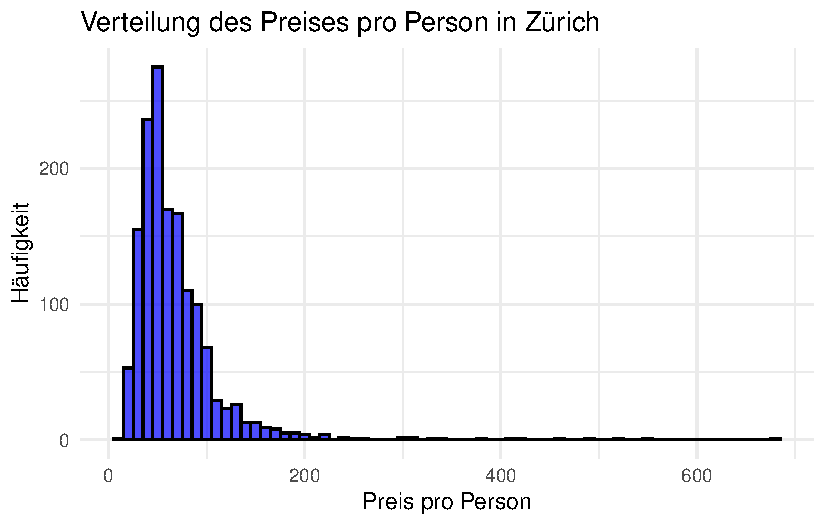
\includegraphics{main_files/figure-pdf/descriptive zurich-1.pdf}

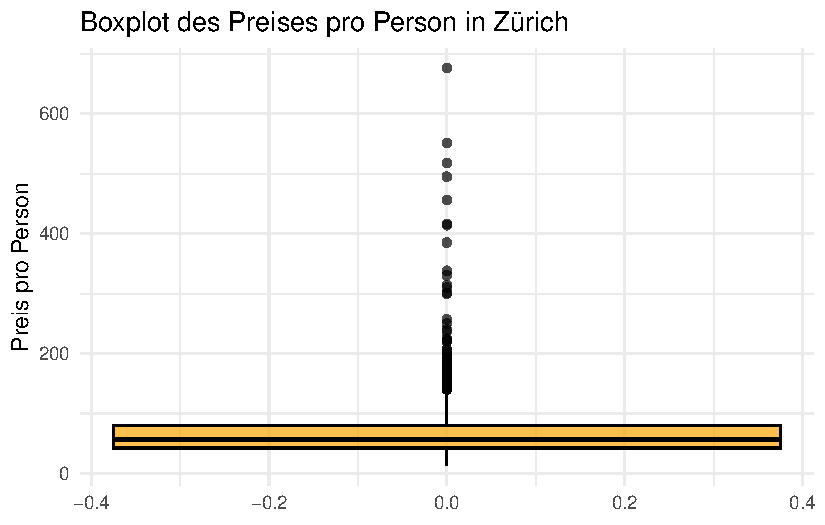
\includegraphics{main_files/figure-pdf/descriptive zurich-2.pdf}

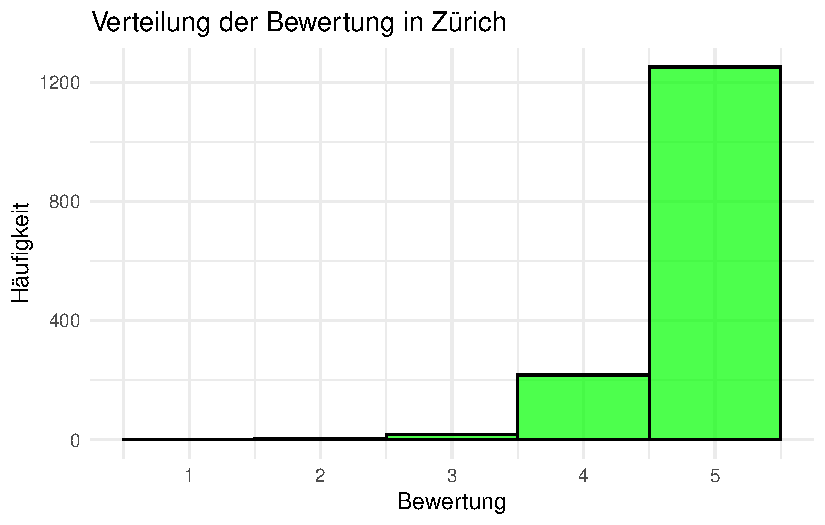
\includegraphics{main_files/figure-pdf/descriptive zurich-3.pdf}

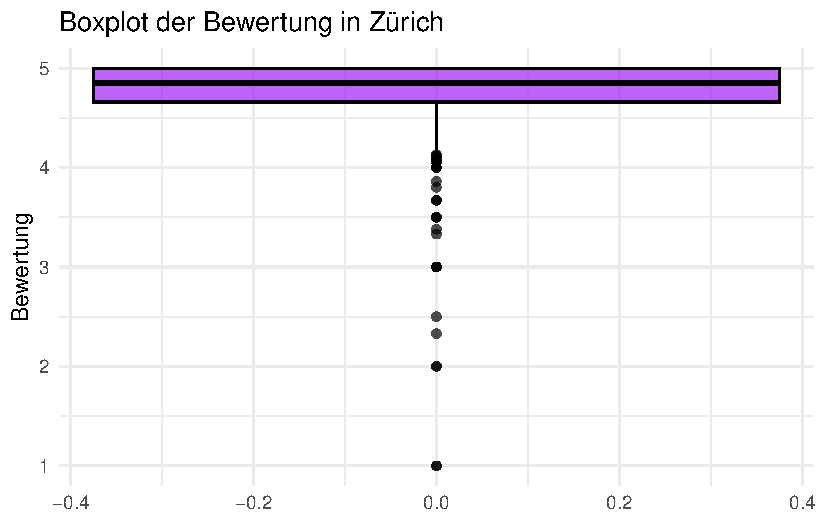
\includegraphics{main_files/figure-pdf/descriptive zurich-4.pdf}

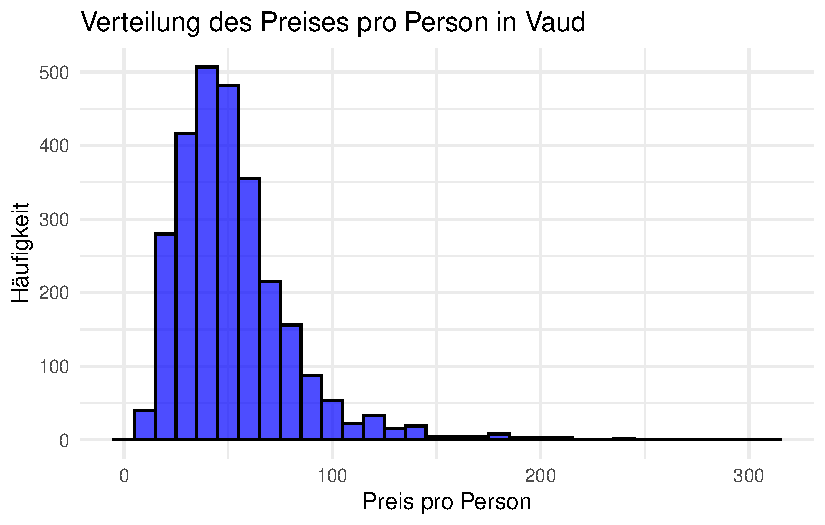
\includegraphics{main_files/figure-pdf/descriptive vaud-1.pdf}

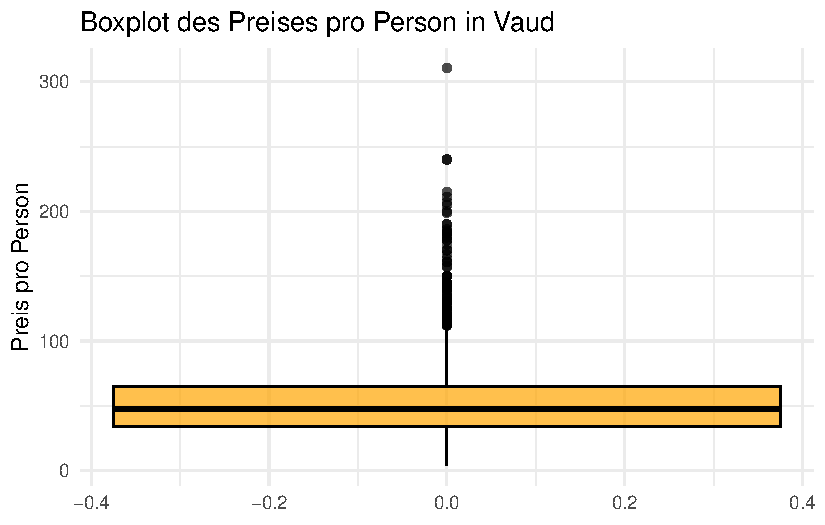
\includegraphics{main_files/figure-pdf/descriptive vaud-2.pdf}

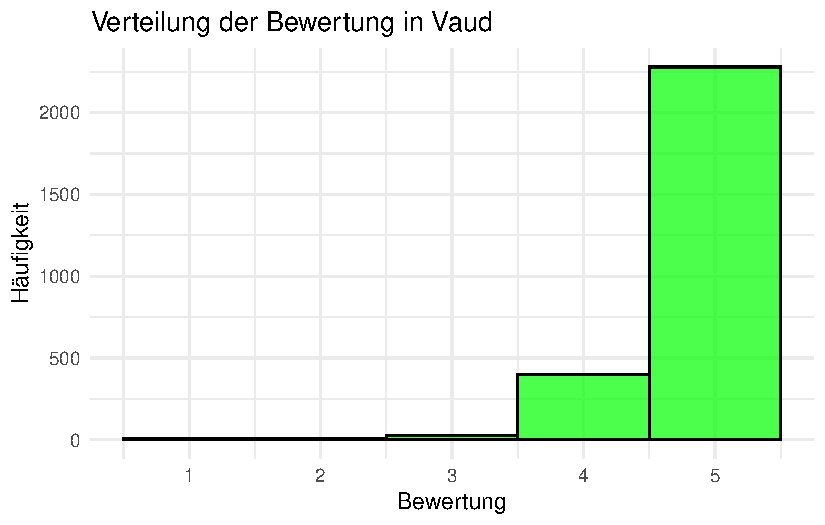
\includegraphics{main_files/figure-pdf/descriptive vaud-3.pdf}

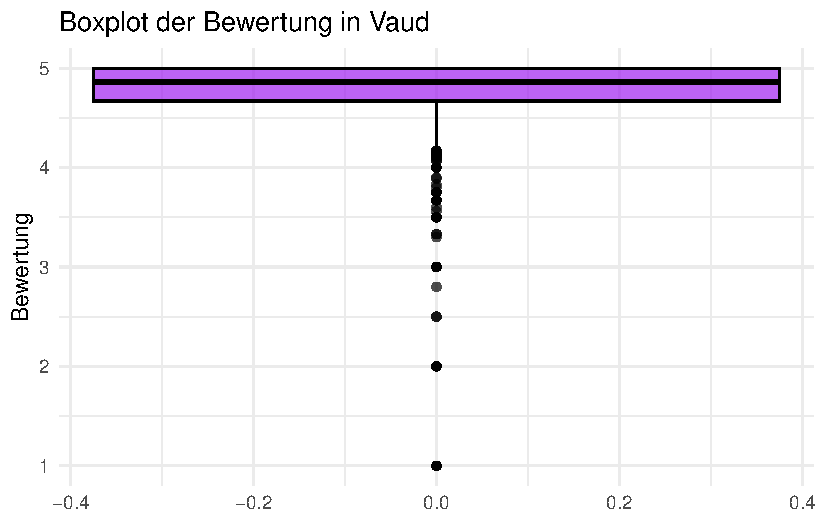
\includegraphics{main_files/figure-pdf/descriptive vaud-4.pdf}

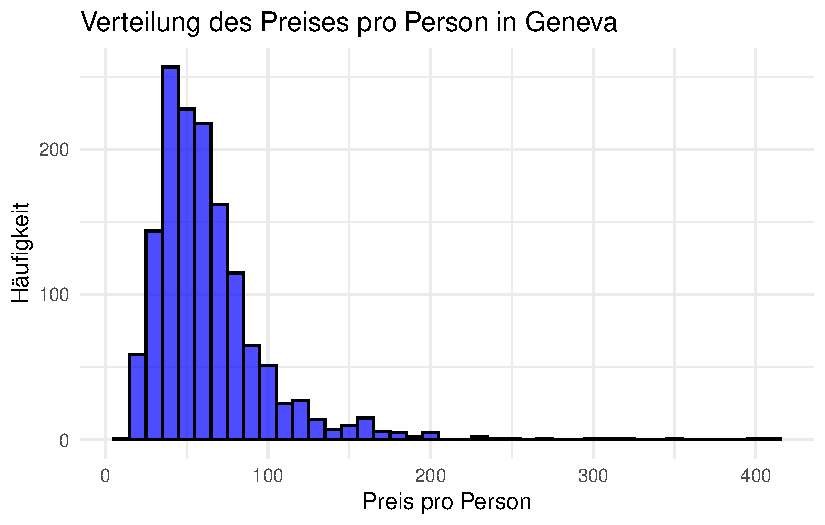
\includegraphics{main_files/figure-pdf/descriptive geneva-1.pdf}

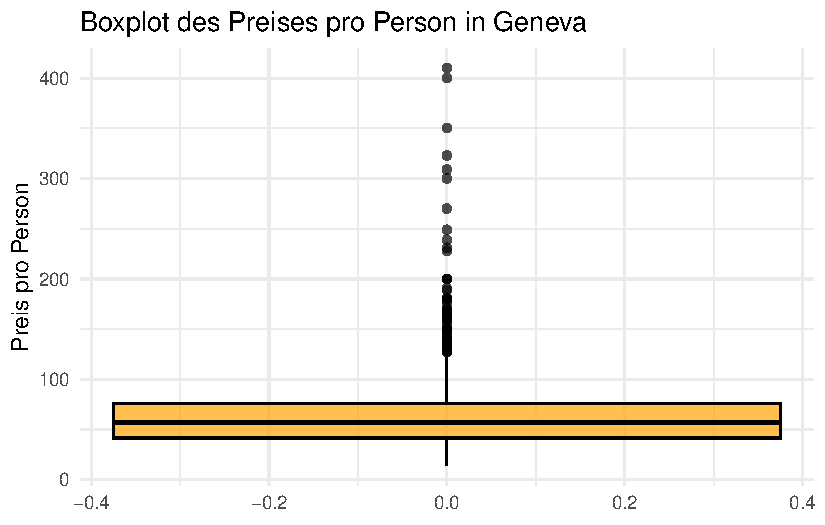
\includegraphics{main_files/figure-pdf/descriptive geneva-2.pdf}

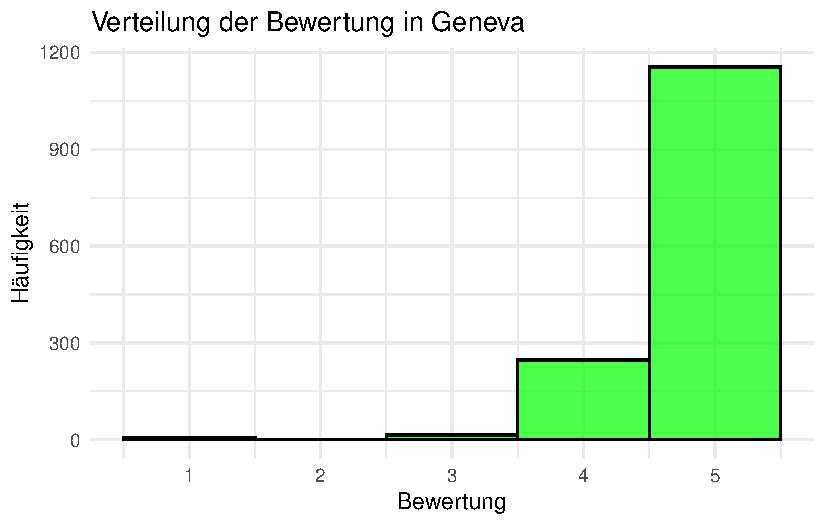
\includegraphics{main_files/figure-pdf/descriptive geneva-3.pdf}

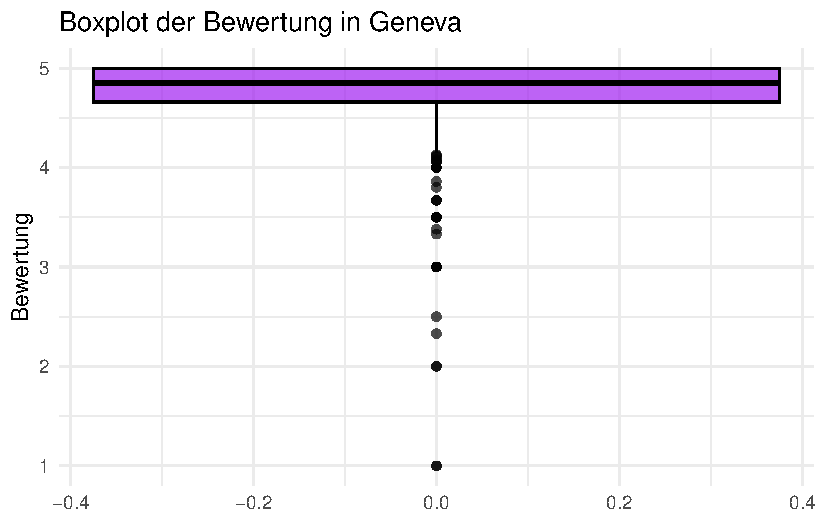
\includegraphics{main_files/figure-pdf/descriptive geneva-4.pdf}

\hypertarget{korrelationsanalyse}{%
\subsubsection{\texorpdfstring{\textbf{Korrelationsanalyse}}{Korrelationsanalyse}}\label{korrelationsanalyse}}

Die Korrelationsanalyse untersucht die Stärke und Richtung der Beziehung
zwischen verschiedenen numerischen Variablen.
Pearson-Korrelationskoeffizienten wurden berechnet, um zu
quantifizieren, wie stark zwei Variablen miteinander variieren. Die Idee
ist, Zusammenhänge zwischen Variablen zu finden, insbesondere zwischen
den Bewertungen, Host-Informationen, geografischen Daten und dem Preis
pro Person. Dafür berechnen wir den Korrelationskoeffizienten und gehen
auf die Top 5 der positiven und negativen Korrelationen ein.

\hypertarget{lineare-regression}{%
\subsubsection{\texorpdfstring{\textbf{Lineare
Regression}}{Lineare Regression}}\label{lineare-regression}}

Die lineare Regression wurde verwendet, um die Beziehung zwischen einer
abhängigen Variable (Preis pro Person) und einer oder mehreren
unabhängigen Variablen zu modellieren. Dies hilft, die Auswirkungen der
unabhängigen Variablen auf die abhängige Variable zu quantifizieren und
Vorhersagen zu treffen. Dafür untersuchen wir den Einfluss einzelner
Variablen (z.B. Bewertungen, Host-Attribute, Entfernung zum
Stadtzentrum) auf den Preis pro Person, um unsere Hypothesen zu
überprüfen. Weiterhin erstellen wir mehrere lineare Regressionsmodelle,
um den Einfluss spezifischer unabhängiger Variablen auf die abhängige
Variable (Preis pro Person) zu analysieren.

\hypertarget{visualisierung}{%
\subsubsection{\texorpdfstring{\textbf{Visualisierung}}{Visualisierung}}\label{visualisierung}}

Verschiedene Arten von Plots wurden verwendet, um die Ergebnisse der
deskriptiven Statistik, der Korrelationsanalyse und der
Regressionsmodelle zu visualisieren. Das Ziel der Visualisierung ist es,
eine verständliche Darstellung der Ergebnisse zu bieten und Muster in
den Daten zu identifizieren.

\hypertarget{predictive-analysis}{%
\subsubsection{\texorpdfstring{\textbf{Predictive
Analysis}}{Predictive Analysis}}\label{predictive-analysis}}

Um prädiktive Analysen einzubeziehen, haben wir eine Vorhersagemodell
entwickelt, um den erzielbaren Preis basierend auf bestimmten Merkmalen
der Unterkünfte zu prognostizieren. Unser Ziel war es, den Trend des
Preises pro Person der Unterkunft aufzuzeigen und zu untersuchen, ob wir
mithilfe der Bewertung und den wichtigsten Eigenschaften einer
Unterkunft eine Prognose über den Preis machen können. Dabei wurden die
sechs besten Variablen mit der höchsten Korrelation im Modell verwendet.

\begin{verbatim}
[1] "Vorhersagemodell für Zürich"
\end{verbatim}

\begin{verbatim}
RMSE: 18.75538 
\end{verbatim}

\begin{verbatim}
MAE: 8.352074 
\end{verbatim}

\begin{verbatim}
R²: 0.7960764 
\end{verbatim}

Die vorliegende Predictive Analyse zielt darauf ab, den Trend des
Preises pro Person einer Unterkunft aufzuzeigen und zu untersuchen, ob
mithilfe der Bewertung und den wichtigsten Eigenschaften einer
Unterkunft eine Prognose über den Preis gemacht werden kann.

Die Modellbewertung zeigt folgende Ergebnisse:

\begin{itemize}
\item
  \textbf{RMSE: 18.75538} -- Der durchschnittliche quadratische Fehler
  beträgt 18.76 USD, was auf relativ geringe Abweichungen zwischen den
  vorhergesagten und tatsächlichen Preisen hinweist.
\item
  \textbf{MAE: 8.352074} -- Der mittlere absolute Fehler beträgt 8.35
  USD, was ebenfalls auf geringe Abweichungen hinweist.
\item
  \textbf{R²: 0.7960764} -- Ein R²-Wert von 0.80 deutet darauf hin, dass
  das Modell die Variation des Preises pro Person gut erklärt und einen
  grossen Teil der Variabilität im Preis vorhersagen kann.
\end{itemize}

Die Merkmalswichtigkeit zeigt, dass der Preis in USD (IncNodePurity =
1279516.0) der wichtigste Prädiktor ist, gefolgt von der Anzahl der
privaten Zimmer in den Angeboten des Gastgebers (IncNodePurity =
416287.9) und der Anzahl der Personen, die die Unterkunft aufnehmen kann
(IncNodePurity = 420585.7). Andere wichtige Merkmale sind die
Verfügbarkeit über 365 Tage (IncNodePurity = 321470.4), die Gesamtanzahl
der Angebote des Gastgebers (IncNodePurity = 234611.4), und die
durchschnittliche maximale Aufenthaltsdauer (IncNodePurity = 188941.3).
Dies zeigt, dass der Preis in USD, die Anzahl der privaten Zimmer, die
Kapazität der Unterkunft und die Verfügbarkeit wesentliche Faktoren bei
der Preisgestaltung sind.

\begin{verbatim}
[1] "Vorhersagemodell für Vaud"
\end{verbatim}

\begin{verbatim}
RMSE: 15.67096 
\end{verbatim}

\begin{verbatim}
MAE: 6.181381 
\end{verbatim}

\begin{verbatim}
R²: 0.7177398 
\end{verbatim}

Die Modellbewertung zeigt folgende Ergebnisse:

\begin{itemize}
\item
  \textbf{RMSE: 15.67096} -- Der durchschnittliche quadratische Fehler
  beträgt 15.67 USD, was auf relativ geringe Abweichungen zwischen den
  vorhergesagten und tatsächlichen Preisen hinweist.
\item
  \textbf{MAE: 6.181381} -- Der mittlere absolute Fehler beträgt 6.18
  USD, was ebenfalls auf geringe Abweichungen hinweist.
\item
  \textbf{R²: 0.7177398} -- Ein R²-Wert von 0.72 deutet darauf hin, dass
  das Modell die Variation des Preises pro Person gut erklärt und einen
  grossen Teil der Variabilität im Preis vorhersagen kann.
\end{itemize}

Die Merkmalswichtigkeit zeigt, dass der Preis in USD (IncNodePurity =
671102.83) der wichtigste Prädiktor ist, gefolgt von der Anzahl der
privaten Zimmer in den Angeboten des Gastgebers (IncNodePurity =
231015.26) und der Kapazität der Unterkunft (IncNodePurity = 315227.40).
Andere wichtige Merkmale sind die Verfügbarkeit über 90 Tage
(IncNodePurity = 125946.08), die geographische Länge (IncNodePurity =
176045.99) und die Anzahl der Betten (IncNodePurity = 95966.35). Dies
zeigt, dass der Preis in USD, die Anzahl der privaten Zimmer, die
Kapazität der Unterkunft und die Verfügbarkeit wesentliche Faktoren bei
der Preisgestaltung sind.

\begin{verbatim}
[1] "Vorhersagemodell für Genf"
\end{verbatim}

\begin{verbatim}
RMSE: 29.24768 
\end{verbatim}

\begin{verbatim}
MAE: 11.75992 
\end{verbatim}

\begin{verbatim}
R²: 0.5316072 
\end{verbatim}

Die Modellbewertung zeigt folgende Ergebnisse:

\begin{itemize}
\item
  \textbf{RMSE: 29.24768} -- Der durchschnittliche quadratische Fehler
  beträgt 29.25 USD, was auf moderate Abweichungen zwischen den
  vorhergesagten und tatsächlichen Preisen hinweist.
\item
  \textbf{MAE: 11.75992} -- Der mittlere absolute Fehler beträgt 11.76
  USD, was auf mittlere Abweichungen hinweist.
\item
  \textbf{R²: 0.5316072} -- Ein R²-Wert von 0.53 deutet darauf hin, dass
  das Modell die Variation des Preises pro Person teilweise erklärt und
  etwa die Hälfte der Variabilität im Preis vorhersagen kann.
\end{itemize}

Die Merkmalswichtigkeit zeigt, dass der Preis in USD (IncNodePurity =
542561.0) der wichtigste Prädiktor ist, gefolgt von der Anzahl der
privaten Zimmer in den Angeboten des Gastgebers (IncNodePurity =
214197.9) und der Kapazität der Unterkunft (IncNodePurity = 237664.3).
Andere wichtige Merkmale sind die Verfügbarkeit über 30 Tage
(IncNodePurity = 108033.9), 60 Tage (IncNodePurity = 115170.7) und 90
Tage (IncNodePurity = 106147.8). Dies zeigt, dass der Preis in USD, die
Anzahl der privaten Zimmer, die Kapazität der Unterkunft und die
Verfügbarkeit wesentliche Faktoren bei der Preisgestaltung sind.

Insgesamt zeigt die Analyse, dass die Modelle für Zürich und Vaud gut
funktionieren, während das Modell für Genf noch Verbesserungspotenzial
hat.

\hypertarget{ergebnisse-statistische-ergebnisse-zahlen-diagramme}{%
\section{Ergebnisse (statistische Ergebnisse, Zahlen,
Diagramme)}\label{ergebnisse-statistische-ergebnisse-zahlen-diagramme}}

\hypertarget{deskriptive-statistik-1}{%
\subsection{\texorpdfstring{\textbf{Deskriptive
Statistik}}{Deskriptive Statistik}}\label{deskriptive-statistik-1}}

\hypertarget{korrelationsanalyse-1}{%
\subsection{\texorpdfstring{\textbf{Korrelationsanalyse}}{Korrelationsanalyse}}\label{korrelationsanalyse-1}}

\hypertarget{zuxfcrich}{%
\subsubsection{Zürich}\label{zuxfcrich}}

\begin{itemize}
\item
  \textbf{Positive Korrelationen:}

  \begin{itemize}
  \tightlist
  \item
    \textbf{\texttt{price\_in\_usd} (0.4542):} Höherer Gesamtpreis →
    höherer Preis pro Person.
  \item
    \textbf{\texttt{calculated\_host\_listings\_count\_private\_rooms}
    (0.2536):} Mehr private Zimmer → höherer Preis pro Person.
  \item
    \textbf{\texttt{maximum\_maximum\_nights} (0.1956) \&
    \texttt{maximum\_nights\_avg\_ntm} (0.1956):} Längere maximale
    Aufenthaltsdauer → höherer Preis pro Person.
  \item
    \textbf{\texttt{availability\_365} (0.1922):} Ganzjährige
    Verfügbarkeit → höherer Preis pro Person.
  \end{itemize}
\item
  \textbf{Negative Korrelationen:}

  \begin{itemize}
  \tightlist
  \item
    \textbf{\texttt{host\_listings\_count} (-0.1772),
    \texttt{calculated\_host\_listings\_count} (-0.1909),
    \texttt{host\_total\_listings\_count} (-0.2006),
    \texttt{calculated\_host\_listings\_count\_entire\_homes}
    (-0.2063):} Mehr Listings → niedrigerer Preis pro Person.
  \item
    \textbf{\texttt{accommodates} (-0.2531):} Mehr Plätze/Betten →
    niedrigerer Preis pro Person.
  \end{itemize}
\end{itemize}

\hypertarget{vaud}{%
\subsubsection{Vaud}\label{vaud}}

\begin{itemize}
\item
  \textbf{Positive Korrelationen:}

  \begin{itemize}
  \tightlist
  \item
    \textbf{\texttt{price\_in\_usd} (0.2369):} Höherer Gesamtpreis →
    höherer Preis pro Person.
  \item
    \textbf{\texttt{calculated\_host\_listings\_count\_private\_rooms}
    (0.1654):} Mehr private Zimmer → höherer Preis pro Person.
  \item
    \textbf{\texttt{availability\_90} (0.1133),
    \texttt{availability\_365} (0.0997), \texttt{availability\_30}
    (0.0891):} Höhere Verfügbarkeit → höherer Preis pro Person.
  \end{itemize}
\item
  \textbf{Negative Korrelationen:}

  \begin{itemize}
  \tightlist
  \item
    \textbf{\texttt{last\_review} (-0.0820):} Länger zurückliegende
    letzte Bewertung → niedrigerer Preis pro Person.
  \item
    \textbf{\texttt{reviews\_per\_month} (-0.1043):} Mehr Bewertungen
    pro Monat → niedrigerer Preis pro Person.
  \item
    \textbf{\texttt{longitude} (-0.1349):} Östlichere Längengrade →
    niedrigerer Preis pro Person.
  \item
    \textbf{\texttt{beds} (-0.2090) \& \texttt{accommodates} (-0.3130):}
    Mehr Betten/Plätze → niedrigerer Preis pro Person.
  \end{itemize}
\end{itemize}

\hypertarget{geneva}{%
\subsubsection{Geneva}\label{geneva}}

\begin{itemize}
\item
  \textbf{Positive Korrelationen:}

  \begin{itemize}
  \tightlist
  \item
    \textbf{\texttt{price\_in\_usd} (0.3902):} Höherer Gesamtpreis →
    höherer Preis pro Person.
  \item
    \textbf{\texttt{calculated\_host\_listings\_count\_private\_rooms}
    (0.2662):} Mehr private Zimmer → höherer Preis pro Person.
  \item
    \textbf{\texttt{availability\_30} (0.2246),
    \texttt{availability\_60} (0.2184), \texttt{availability\_90}
    (0.1991):} Höhere Verfügbarkeit → höherer Preis pro Person.
  \end{itemize}
\item
  \textbf{Negative Korrelationen:}

  \begin{itemize}
  \tightlist
  \item
    \textbf{\texttt{maximum\_minimum\_nights} (-0.0907):} Höhere
    minimale Aufenthaltsdauer → niedrigerer Preis pro Person.
  \item
    \textbf{\texttt{number\_of\_reviews\_l30d} (-0.0957):} Mehr
    Bewertungen in den letzten 30 Tagen → niedrigerer Preis pro Person.
  \item
    \textbf{\texttt{minimum\_maximum\_nights} (-0.0966):} Höhere
    minimale maximale Aufenthaltsdauer → niedrigerer Preis pro Person.
  \item
    \textbf{\texttt{reviews\_per\_month} (-0.0976):} Mehr Bewertungen
    pro Monat → niedrigerer Preis pro Person.
  \item
    \textbf{\texttt{accommodates} (-0.2185):} Mehr Plätze/Betten →
    niedrigerer Preis pro Person.
  \end{itemize}
\end{itemize}

\hypertarget{gesamtschlussfolgerungen}{%
\subsubsection{Gesamtschlussfolgerungen}\label{gesamtschlussfolgerungen}}

Die Analyse der Korrelationen von \texttt{price\_per\_person} mit
verschiedenen Variablen in den Städten Zürich, Vaud und Geneva liefert
wertvolle Einblicke in die Faktoren, die den Preis pro Person
beeinflussen. Hier sind die ausführlicheren Schlussfolgerungen:

\begin{itemize}
\item
  \textbf{Höherer Gesamtpreis (\texttt{price\_in\_usd})}: In allen drei
  Städten besteht ein positiver Zusammenhang zwischen dem Gesamtpreis
  und dem Preis pro Person. Das bedeutet, dass teurere Wohnungen auch
  mehr pro Person kosten. Dies ist intuitiv nachvollziehbar, da eine
  höhere Grundmiete oft auch zu höheren Kosten pro Person führt. Das
  bedeutet aber auch, dass man, wenn man mit einer grösseren Gruppe
  reist und eine grössere Unterkunft mietet, pro Person weniger zahlt.
\item
  \textbf{Mehr private Zimmer
  (\texttt{calculated\_host\_listings\_count\_private\_rooms})}:
  Ebenfalls in allen drei Städten korreliert die Anzahl der privaten
  Zimmer im Angebot des Hosts positiv mit dem Preis pro Person. Dies
  könnte darauf hinweisen, dass Hosts, die mehr private Zimmer anbieten,
  tendenziell höhere Preise verlangen, möglicherweise aufgrund der
  höheren Privatsphäre und Exklusivität.
\item
  \textbf{Kurzfristige und langfristige Verfügbarkeit}: In Geneva und
  Vaud zeigt die Verfügbarkeit der Unterkunft über verschiedene
  Zeiträume (30, 60, 90 Tage und das ganze Jahr) eine positive
  Korrelation mit dem Preis pro Person. Dies deutet darauf hin, dass
  Unterkünfte, die sowohl kurzfristig als auch langfristig verfügbar
  sind, tendenziell höher bepreist werden. Es könnte sein, dass diese
  Unterkünfte eine höhere Nachfrage bedienen oder flexiblere
  Buchungsoptionen bieten, die höher bewertet werden.
\item
  \textbf{Häufigkeit der Bewertungen (\texttt{reviews\_per\_month},
  \texttt{number\_of\_reviews\_l30d})}: In Vaud und Geneva gibt es eine
  negative Korrelation zwischen der Anzahl der Bewertungen pro Monat und
  dem Preis pro Person. Dies könnte darauf hindeuten, dass Unterkünfte,
  die häufiger bewertet werden, tendenziell günstiger sind. Diese
  Unterkünfte könnten eine breitere Zielgruppe ansprechen,
  einschliesslich preisbewusster Reisender, was zu häufigeren Buchungen
  und somit zu mehr Bewertungen führt.
\item
  \textbf{Zeit seit der letzten Bewertung (\texttt{last\_review})}: In
  Vaud zeigt sich eine leichte negative Korrelation zwischen der Zeit
  seit der letzten Bewertung und dem Preis pro Person. Dies könnte
  darauf hinweisen, dass aktuellere Bewertungen mit höheren Preisen pro
  Person verbunden sind, möglicherweise weil aktuelle Bewertungen das
  Vertrauen und die Attraktivität der Unterkunft erhöhen.
\item
  \textbf{Anzahl der Listings (\texttt{host\_listings\_count},
  \texttt{calculated\_host\_listings\_count},
  \texttt{host\_total\_listings\_count},
  \texttt{calculated\_host\_listings\_count\_entire\_homes})}: In Zürich
  zeigen mehrere Variablen, die die Anzahl der Listings des Hosts
  messen, eine negative Korrelation mit dem Preis pro Person. Dies
  deutet darauf hin, dass Hosts mit vielen Listings ihre Preise
  wettbewerbsfähiger gestalten müssen, um die Nachfrage zu halten.
  Grössere Host-Operationen könnten Skaleneffekte nutzen, um niedrigere
  Preise anzubieten.
\item
  \textbf{Anzahl der Betten und verfügbare Plätze (\texttt{beds},
  \texttt{accommodates})}: In allen drei Städten zeigen sich negative
  Korrelationen zwischen der Anzahl der Betten bzw. der verfügbaren
  Plätze und dem Preis pro Person. Dies weist darauf hin, dass grössere
  Unterkünfte tendenziell niedrigere Pro-Kopf-Kosten haben. Dies könnte
  auf Skaleneffekte oder die Notwendigkeit, grössere Gruppen anzuziehen,
  zurückzuführen sein.
\item
  \textbf{Geografische Koordinaten (\texttt{longitude},
  \texttt{latitude})}: In Vaud zeigt der Längengrad eine signifikante
  negative Korrelation mit dem Preis pro Person, was auf eine
  geografische Preisstruktur hindeuten könnte. Dies könnte bedeuten,
  dass östlichere Lagen tendenziell günstiger sind. In Zürich und Geneva
  sind die geografischen Koordinaten nicht signifikant.
\end{itemize}

\hypertarget{lineare-regression-1}{%
\subsection{\texorpdfstring{\textbf{Lineare
Regression}}{Lineare Regression}}\label{lineare-regression-1}}

\hypertarget{bewertung-der-airbnb-unterkuxfcnfte}{%
\subsubsection{Bewertung der
Airbnb-Unterkünfte}\label{bewertung-der-airbnb-unterkuxfcnfte}}

\textbf{Hypothesen:}

\begin{itemize}
\tightlist
\item
  Nullhypothese (H0): Die Höhe der Gesamtbewertung
  (review\_scores\_rating) hat keinen signifikanten Einfluss auf den
  Preis pro Person der Unterkunft.
\item
  Alternativhypothese (H1): Die Höhe der Gesamtbewertung
  (review\_scores\_rating) hat einen signifikanten Einfluss auf den
  Preis pro Person der Unterkunft.
\end{itemize}

\textbf{Ergebnisse:}

\textbf{Zürich:}

\begin{itemize}
\item
  \texttt{review\_scores\_rating}: Nicht signifikant (p = 0.9598)
\item
  \texttt{review\_scores\_cleanliness}: Signifikant (p = 0.0126) mit
  positivem Einfluss (Estimate = 12.9328)
\item
  \texttt{review\_scores\_communication}: Nicht signifikant (p = 0.5146)
\item
  \textbf{Interpretation:} Die Sauberkeitsbewertung beeinflusst den
  Preis pro Person positiv und signifikant, während die Gesamtbewertung
  und die Kommunikationsbewertung keinen signifikanten Einfluss haben.
\end{itemize}

\textbf{Vaud:}

\begin{itemize}
\item
  \texttt{review\_scores\_rating}: Nicht signifikant (p = 0.6718)
\item
  \texttt{review\_scores\_cleanliness}: Signifikant (p = 3.40e-05) mit
  positivem Einfluss (Estimate = 8.596)
\item
  \texttt{review\_scores\_communication}: Signifikant (p = 0.0177) mit
  negativem Einfluss (Estimate = -5.619)
\item
  \textbf{Interpretation:} In Vaud hat die Sauberkeitsbewertung einen
  signifikanten positiven Einfluss, während die Kommunikationsbewertung
  einen signifikanten negativen Einfluss auf den Preis pro Person hat.
  Die Gesamtbewertung ist nicht signifikant.
\end{itemize}

\textbf{Geneva:}

\begin{itemize}
\item
  \texttt{review\_scores\_rating}: Nicht signifikant (p = 0.1512)
\item
  \texttt{review\_scores\_cleanliness}: Signifikant (p = 0.0002) mit
  positivem Einfluss (Estimate = 14.473)
\item
  \texttt{review\_scores\_communication}: Grenzwertig signifikant (p =
  0.0809) mit negativem Einfluss (Estimate = -6.894)
\item
  \textbf{Interpretation:} In Geneva hat die Sauberkeitsbewertung einen
  signifikanten positiven Einfluss auf den Preis pro Person, während die
  Gesamtbewertung keinen signifikanten Einfluss hat. Die
  Kommunikationsbewertung ist grenzwertig signifikant negativ.
\end{itemize}

\hypertarget{gastgeber-der-airbnb-unterkunft}{%
\subsubsection{Gastgeber der
Airbnb-Unterkunft}\label{gastgeber-der-airbnb-unterkunft}}

\textbf{Hypothesen:}

\begin{itemize}
\tightlist
\item
  Nullhypothese (H0): Die Attribute des Hosts wie
  ``host\_is\_superhost'', ``host\_identity\_verified'' und
  ``host\_listings\_count'' haben keinen signifikanten Einfluss auf den
  Preis pro Person der Unterkunft.
\item
  Alternativhypothese (H1): Die Attribute des Hosts wie
  ``host\_is\_superhost'', ``host\_identity\_verified'' und
  ``host\_listings\_count'' haben einen signifikanten Einfluss auf den
  Preis pro Person der Unterkunft.
\end{itemize}

\textbf{Ergebnisse:}

\textbf{Zürich:}

\begin{itemize}
\item
  \texttt{host\_is\_superhost}: Grenzwertig signifikant (p = 0.0931)
\item
  \texttt{host\_identity\_verified}: Grenzwertig signifikant (p =
  0.0611) mit negativem Einfluss (Estimate = -14.39683)
\item
  \texttt{host\_listings\_count}: Signifikant (p = 3.03e-10) mit
  negativem Einfluss (Estimate = -0.12963)
\item
  \textbf{Interpretation:} In Zürich hat die Anzahl der Listings eines
  Hosts einen signifikant negativen Einfluss auf den Preis pro Person.
  Der Status ``Superhost'' und die Verifizierung des Hosts sind
  grenzwertig signifikant.
\end{itemize}

\textbf{Vaud:}

\begin{itemize}
\item
  \texttt{host\_is\_superhost}: Nicht signifikant (p = 0.8962)
\item
  \texttt{host\_identity\_verified}: Grenzwertig signifikant (p =
  0.0927) mit negativem Einfluss (Estimate = -4.994676)
\item
  \texttt{host\_listings\_count}: Nicht signifikant (p = 0.4207)
\item
  \textbf{Interpretation:} In Vaud sind keine der Host-Attribute
  signifikant, jedoch ist die Verifizierung des Hosts grenzwertig
  signifikant negativ.
\end{itemize}

\textbf{Geneva:}

\begin{itemize}
\item
  \texttt{host\_is\_superhost}: Nicht signifikant (p = 0.206)
\item
  \texttt{host\_identity\_verified}: Nicht signifikant (p = 0.281)
\item
  \texttt{host\_listings\_count}: Nicht signifikant (p = 0.533)
\item
  \textbf{Interpretation:} In Geneva haben die Host-Attribute keinen
  signifikanten Einfluss auf den Preis pro Person.
\end{itemize}

\hypertarget{lage-des-airbnb}{%
\subsubsection{Lage des Airbnb}\label{lage-des-airbnb}}

\textbf{Hypothesen:}

\begin{itemize}
\tightlist
\item
  Nullhypothese (H0): Die Entfernung zum Stadtzentrum (berechnet durch
  geografische Koordinaten) hat keinen signifikanten Einfluss auf den
  Preis pro Person der Unterkunft.
\item
  Alternativhypothese (H1): Die Entfernung zum Stadtzentrum (berechnet
  durch geografische Koordinaten) hat einen signifikanten Einfluss auf
  den Preis pro Person der Unterkunft.
\end{itemize}

\textbf{Ergebnisse:}

\textbf{Zürich:}

\begin{itemize}
\item
  \texttt{longitude}: Nicht signifikant (p = 0.235)
\item
  \texttt{latitude}: Nicht signifikant (p = 0.159)
\item
  \textbf{Interpretation:} Die geografischen Koordinaten haben keinen
  signifikanten Einfluss auf den Preis pro Person in Zürich.
\end{itemize}

\textbf{Vaud:}

\begin{itemize}
\item
  \texttt{longitude}: Signifikant (p = 2.05e-12) mit negativem Einfluss
  (Estimate = -16.129)
\item
  \texttt{latitude}: Nicht signifikant (p = 0.2062)
\item
  \textbf{Interpretation:} In Vaud hat der Längengrad einen
  signifikanten negativen Einfluss auf den Preis pro Person, während der
  Breitengrad keinen signifikanten Einfluss hat.
\end{itemize}

\textbf{Geneva:}

\begin{itemize}
\item
  \texttt{longitude}: Nicht signifikant (p = 0.611)
\item
  \texttt{latitude}: Nicht signifikant (p = 0.396)
\item
  \textbf{Interpretation:} In Geneva haben die geografischen Koordinaten
  keinen signifikanten Einfluss auf den Preis pro Person.
\end{itemize}

\hypertarget{zusammenfassung}{%
\subsection{Zusammenfassung:}\label{zusammenfassung}}

\begin{itemize}
\tightlist
\item
  \textbf{Bewertung:} Die Sauberkeitsbewertung hat in allen Städten
  einen signifikanten positiven Einfluss auf den Preis pro Person. Die
  Gesamtbewertung hat keinen signifikanten Einfluss. Die
  Kommunikationsbewertung hat in Vaud einen signifikanten negativen
  Einfluss.
\item
  \textbf{Gastgeber:} In Zürich hat die Anzahl der Listings eines Hosts
  einen signifikant negativen Einfluss. In Vaud und Geneva sind die
  Host-Attribute nicht signifikant.
\item
  \textbf{Lage:} In Vaud hat der Längengrad einen signifikanten
  negativen Einfluss auf den Preis pro Person. In Zürich und Geneva
  haben die geografischen Koordinaten keinen signifikanten Einfluss.
\end{itemize}

\hypertarget{visualisierung-1}{%
\subsection{\texorpdfstring{\textbf{Visualisierung}}{Visualisierung}}\label{visualisierung-1}}

Die folgenden Plots zeigen die Korrelationen des Preis pro Person
(\texttt{price\_per\_person}) in den verschiedenen Städten. Anhand
dieser Diagramme lässt sich leicht erkennen, dass einige Korrelationen
viel stärker positiv oder negativ ausfallen. Diese starken Korrelationen
sollten genauer untersucht werden, um ihre Ursachen und Auswirkungen
besser zu verstehen.

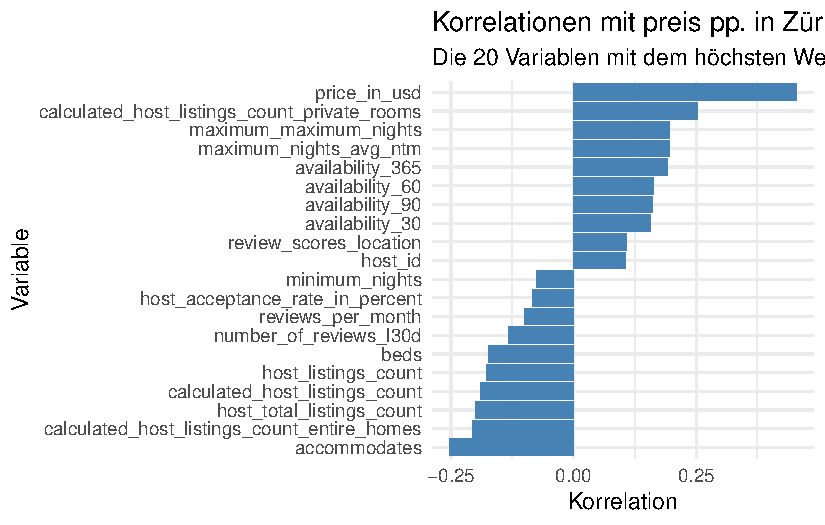
\includegraphics{main_files/figure-pdf/unnamed-chunk-12-1.pdf}

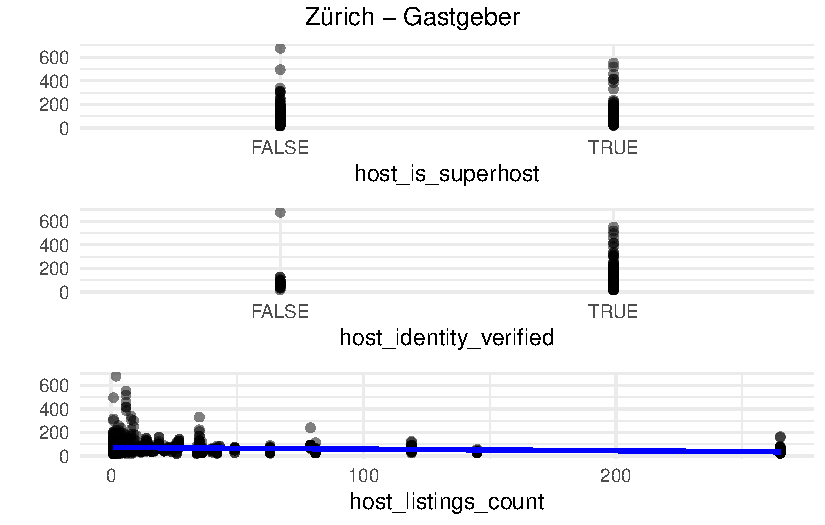
\includegraphics{main_files/figure-pdf/unnamed-chunk-12-2.pdf}

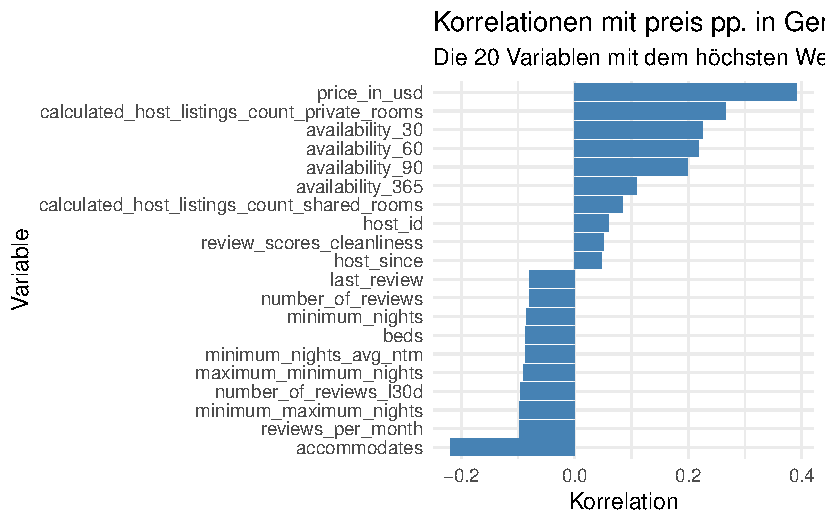
\includegraphics{main_files/figure-pdf/unnamed-chunk-12-3.pdf}

\hypertarget{lineare-regression-fuxfcr-zuxfcrich}{%
\subsubsection{Lineare Regression für
Zürich}\label{lineare-regression-fuxfcr-zuxfcrich}}

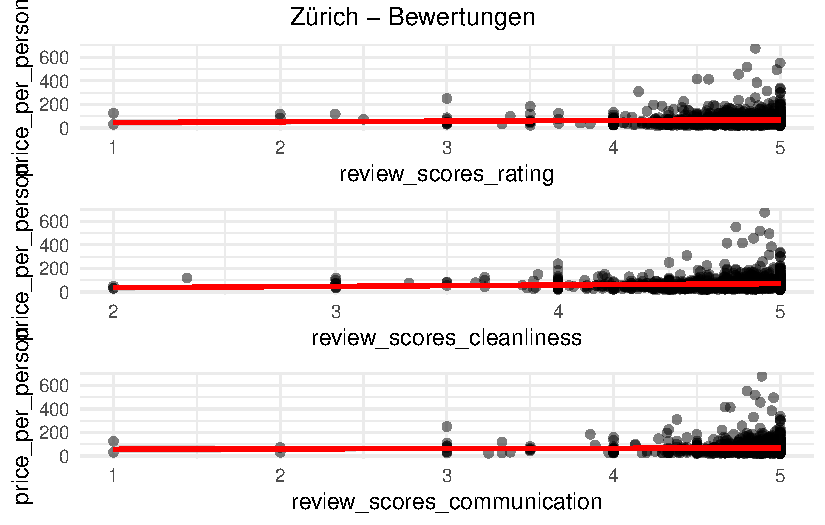
\includegraphics{main_files/figure-pdf/unnamed-chunk-13-1.pdf}

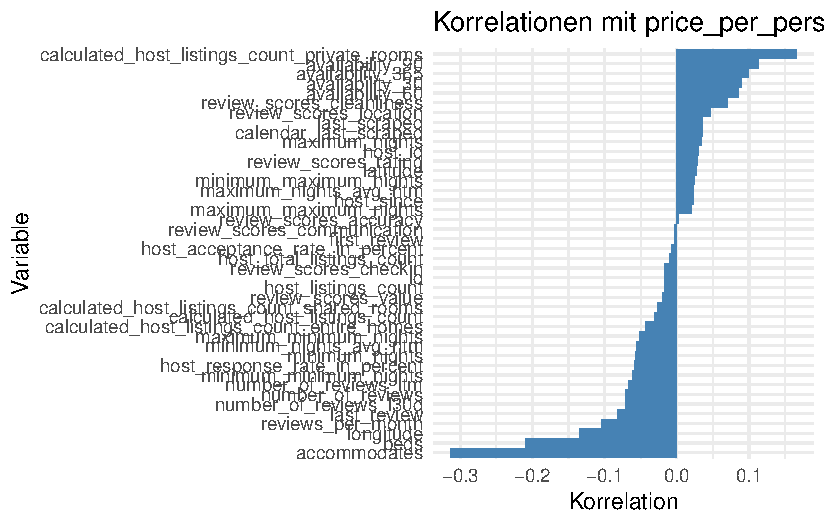
\includegraphics{main_files/figure-pdf/unnamed-chunk-13-2.pdf}

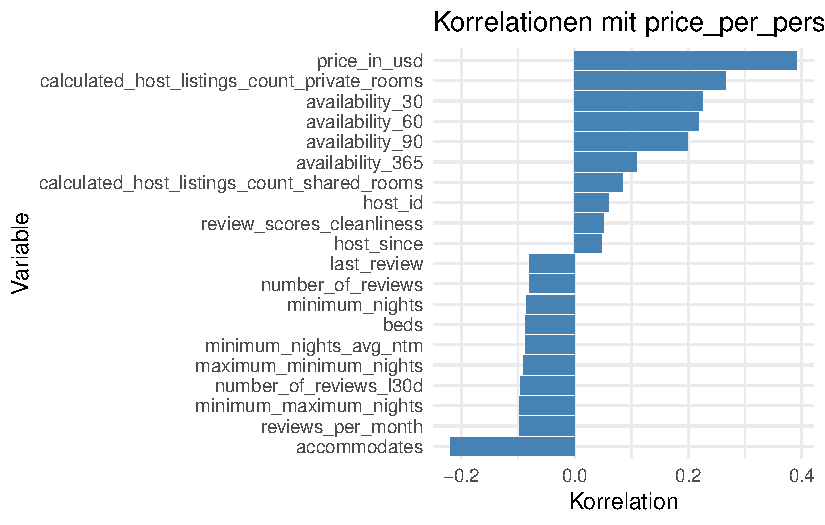
\includegraphics{main_files/figure-pdf/unnamed-chunk-13-3.pdf}

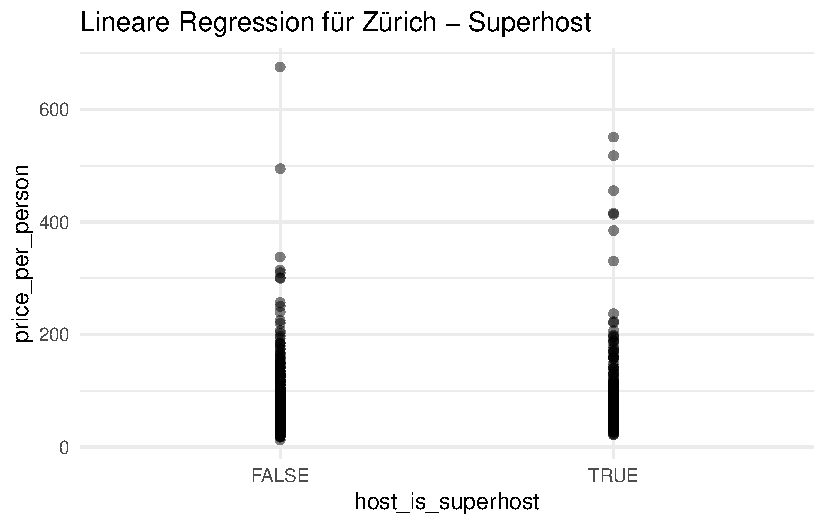
\includegraphics{main_files/figure-pdf/unnamed-chunk-13-4.pdf}

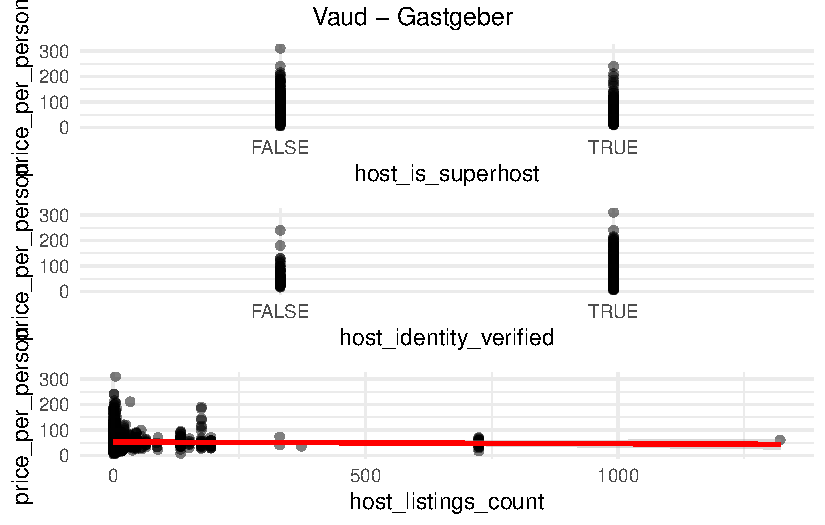
\includegraphics{main_files/figure-pdf/unnamed-chunk-13-5.pdf}

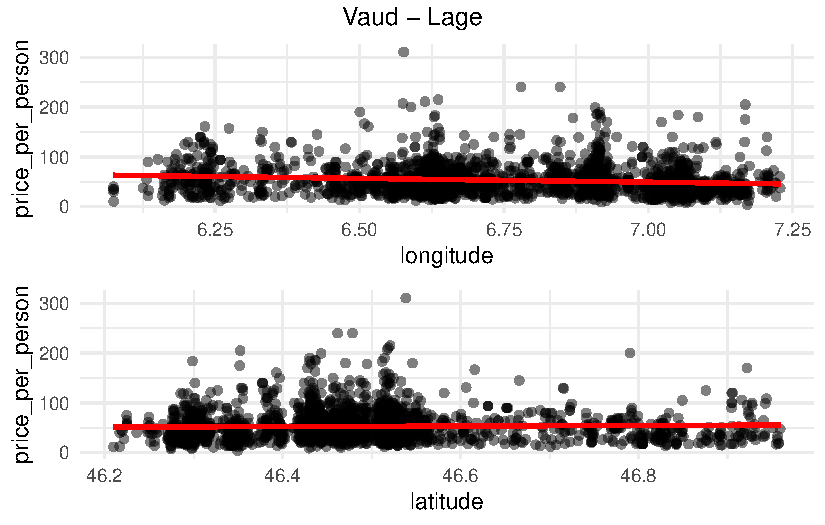
\includegraphics{main_files/figure-pdf/unnamed-chunk-13-6.pdf}

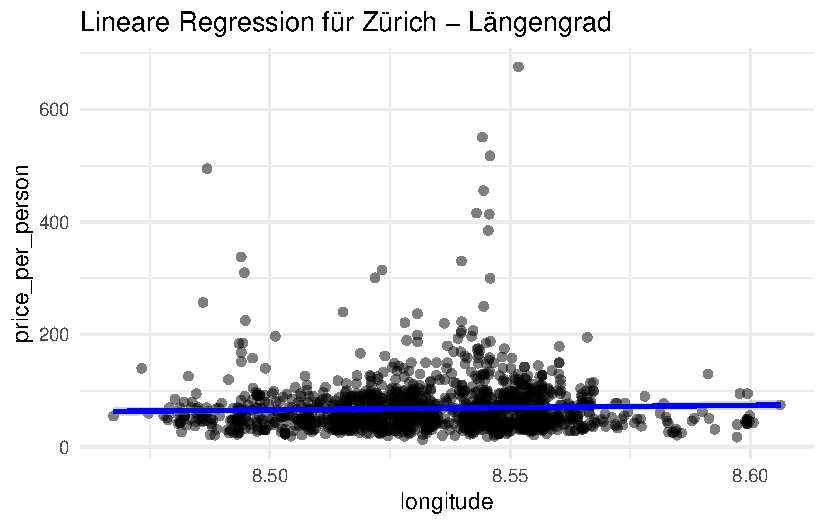
\includegraphics{main_files/figure-pdf/unnamed-chunk-13-7.pdf}

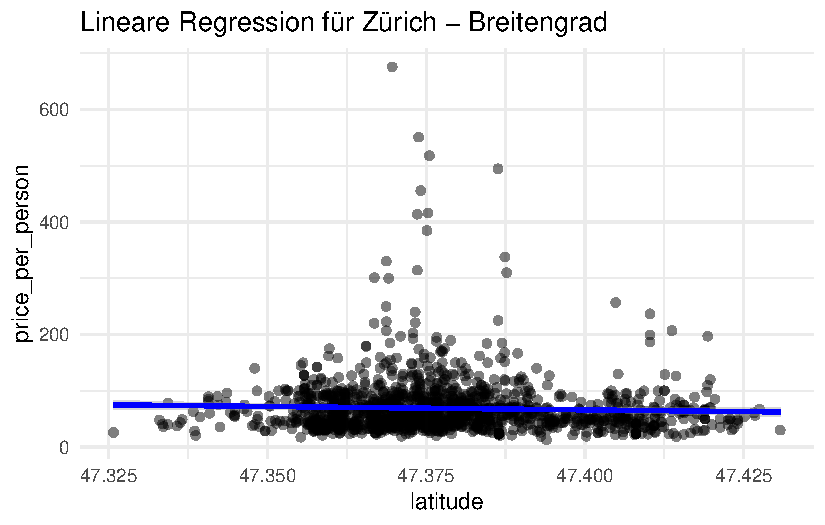
\includegraphics{main_files/figure-pdf/unnamed-chunk-13-8.pdf}

\hypertarget{lineare-regression-fuxfcr-vaud}{%
\subsubsection{Lineare Regression für
Vaud}\label{lineare-regression-fuxfcr-vaud}}

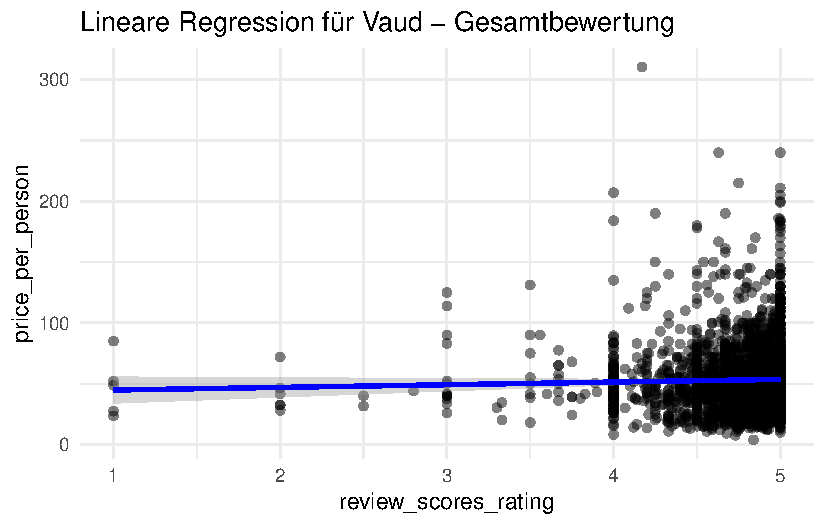
\includegraphics{main_files/figure-pdf/unnamed-chunk-14-1.pdf}

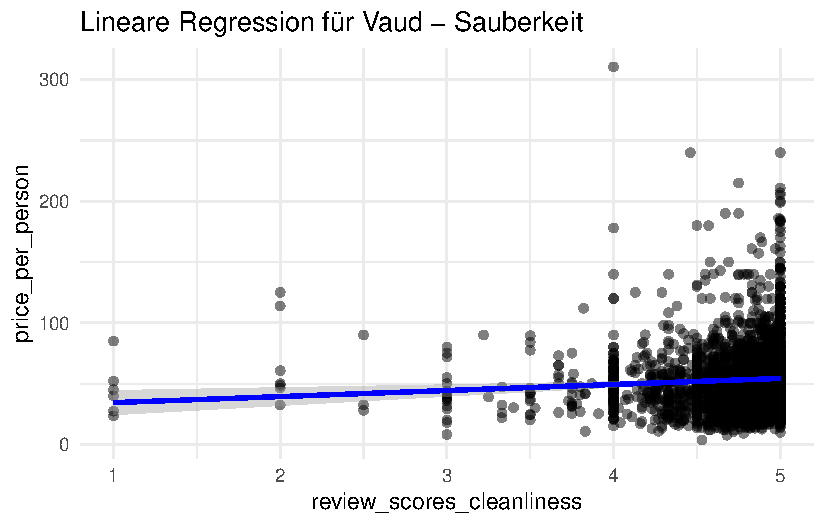
\includegraphics{main_files/figure-pdf/unnamed-chunk-14-2.pdf}

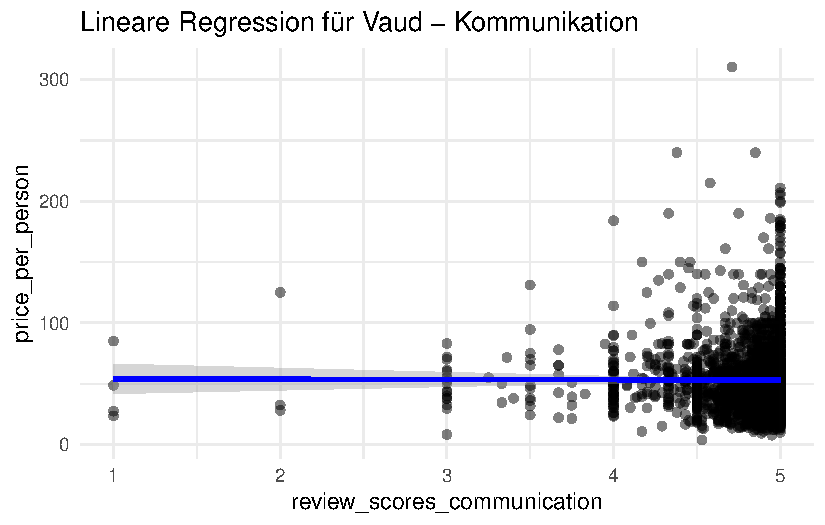
\includegraphics{main_files/figure-pdf/unnamed-chunk-14-3.pdf}

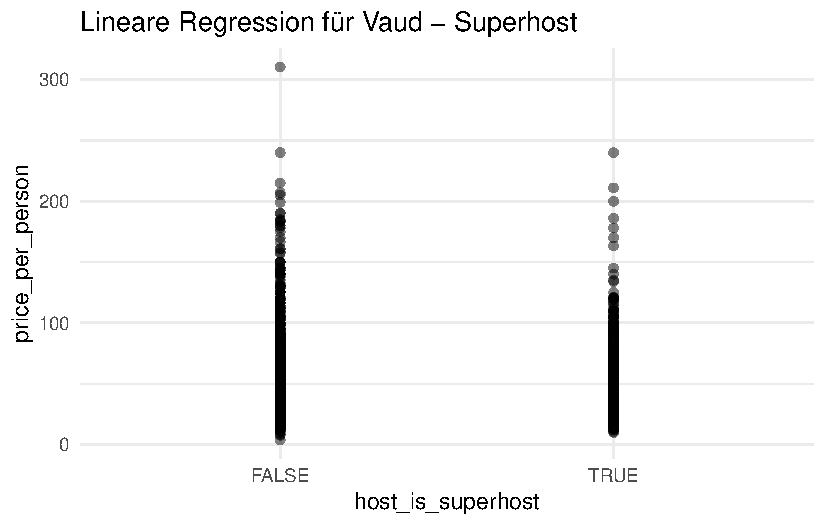
\includegraphics{main_files/figure-pdf/unnamed-chunk-14-4.pdf}

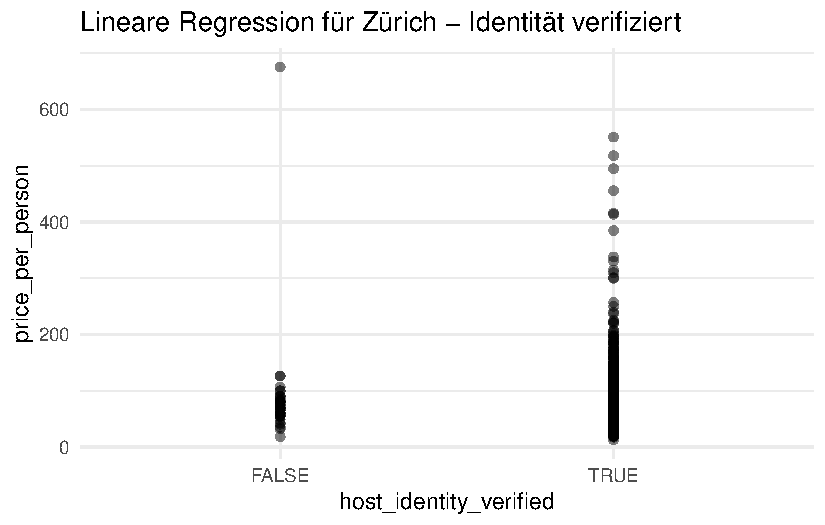
\includegraphics{main_files/figure-pdf/unnamed-chunk-14-5.pdf}

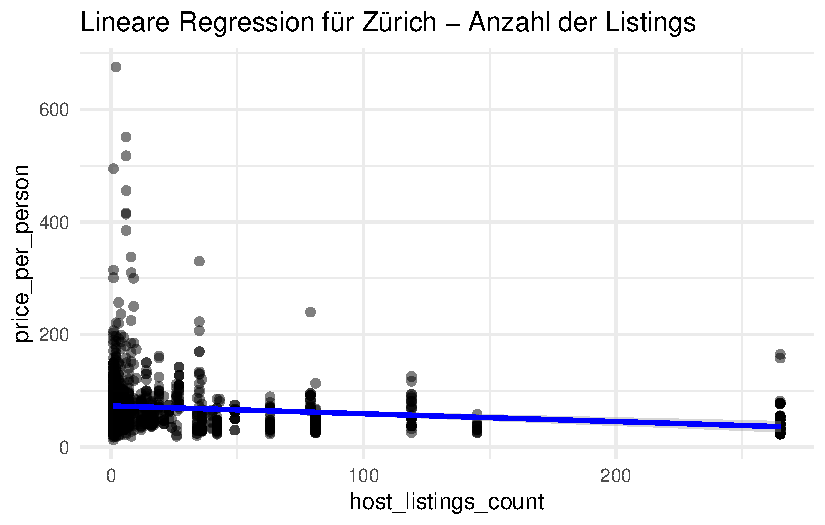
\includegraphics{main_files/figure-pdf/unnamed-chunk-14-6.pdf}

\hypertarget{lineare-regression-fuxfcr-geneva}{%
\subsubsection{Lineare Regression für
Geneva}\label{lineare-regression-fuxfcr-geneva}}

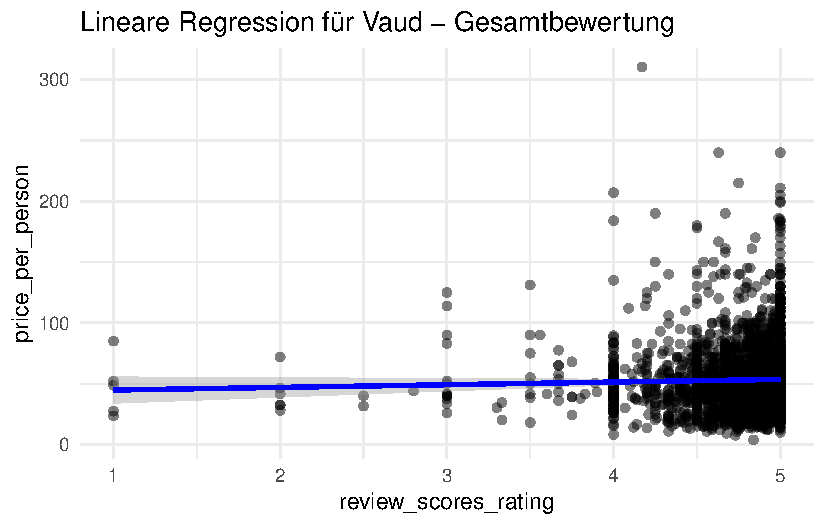
\includegraphics{main_files/figure-pdf/unnamed-chunk-15-1.pdf}

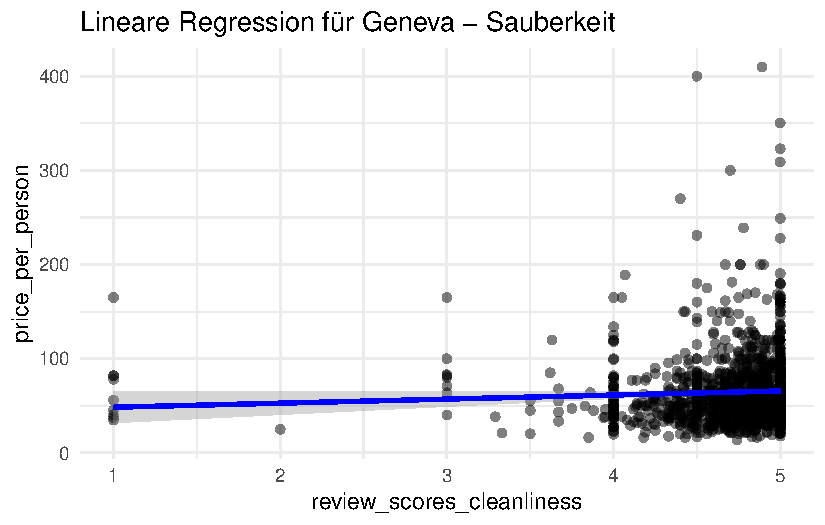
\includegraphics{main_files/figure-pdf/unnamed-chunk-15-2.pdf}

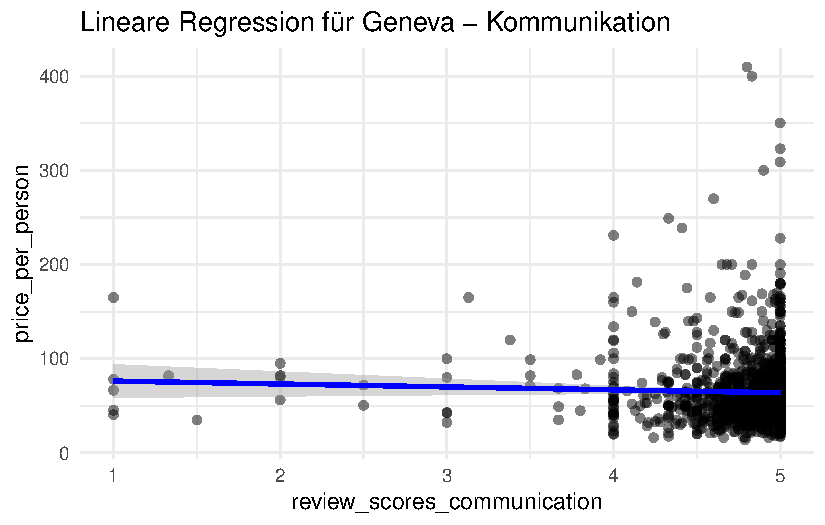
\includegraphics{main_files/figure-pdf/unnamed-chunk-15-3.pdf}

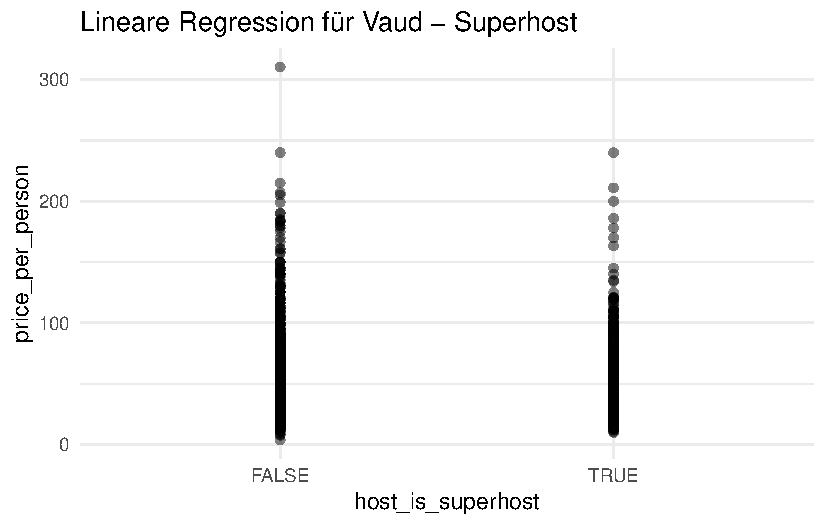
\includegraphics{main_files/figure-pdf/unnamed-chunk-15-4.pdf}

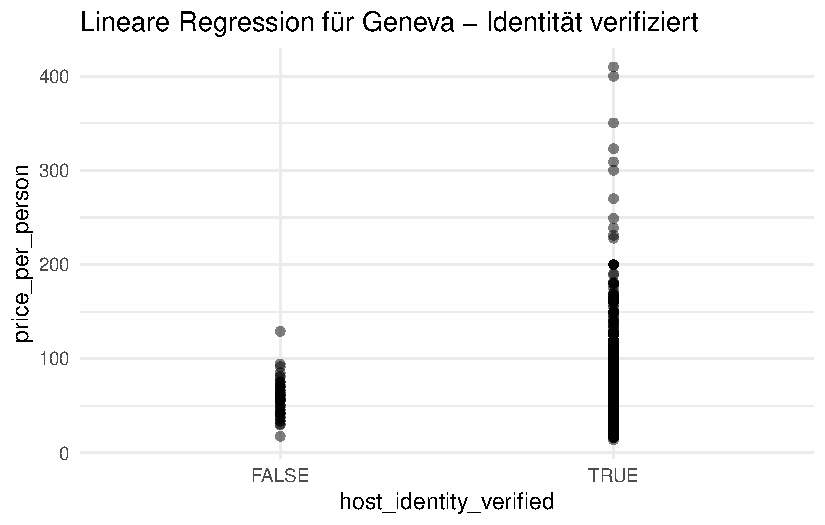
\includegraphics{main_files/figure-pdf/unnamed-chunk-15-5.pdf}

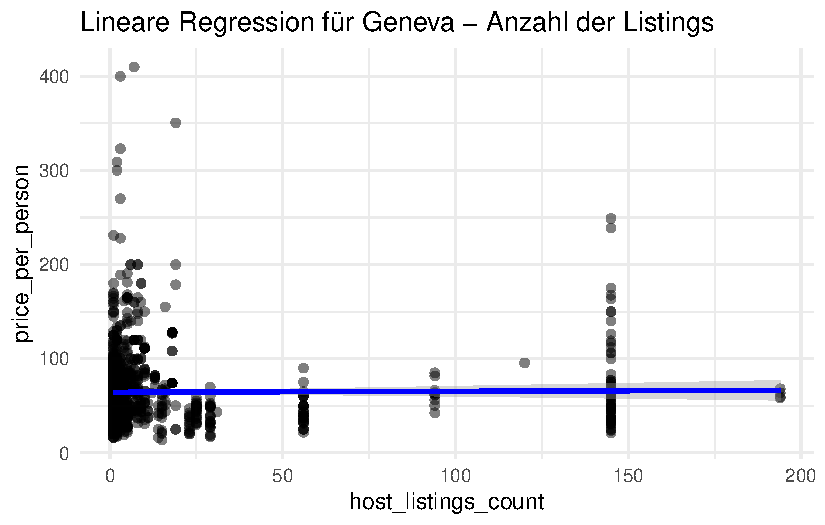
\includegraphics{main_files/figure-pdf/unnamed-chunk-15-6.pdf}

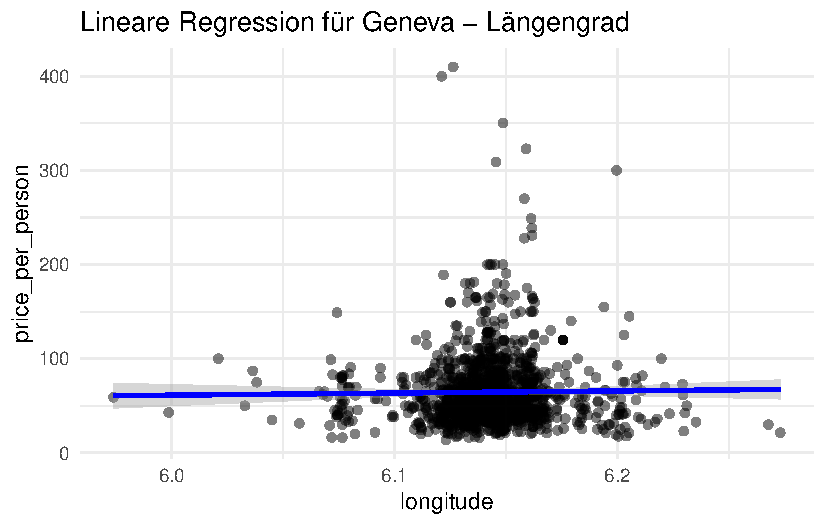
\includegraphics{main_files/figure-pdf/unnamed-chunk-15-7.pdf}

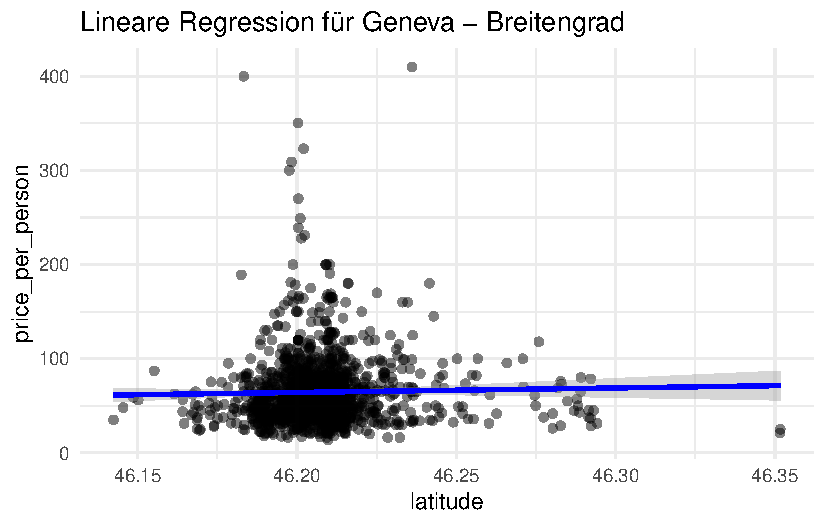
\includegraphics{main_files/figure-pdf/unnamed-chunk-15-8.pdf}

\hypertarget{schlussfolgerung}{%
\subsubsection{Schlussfolgerung}\label{schlussfolgerung}}

Die verschiedenen Grafiken und deren lineare Regressionen liefern
interessante Einblicke in die Beziehung zwischen den untersuchten
Variablen und dem Preis pro Person. Allerdings zeigen die Ergebnisse,
dass viele der unabhängigen Variablen nur einen geringen Einfluss auf
den Preis pro Person haben.

Zusammenfassend lässt sich sagen, dass die meisten untersuchten
Variablen keinen starken Einfluss auf den Preis pro Person haben. Dies
könnte darauf hindeuten, dass andere, nicht berücksichtigte Faktoren
eine grössere Rolle spielen oder dass die Märkte in diesen Städten
relativ homogen sind. Weitere Untersuchungen könnten sich auf
zusätzliche Variablen oder nicht-lineare Modelle konzentrieren, um
potenzielle Einflussfaktoren besser zu identifizieren.

\hypertarget{predictive-analysis-1}{%
\subsection{Predictive Analysis}\label{predictive-analysis-1}}

Um prädiktive Analysen einzubeziehen, haben wir ein Vorhersagemodell
entwickelt, um den erzielbaren Preis basierend auf bestimmten Merkmalen
der Unterkünfte zu prognostizieren. Unser Ziel war es, den Trend des
Preises pro Person der Unterkunft aufzuzeigen und zu untersuchen, ob wir
mithilfe der Bewertung und den wichtigsten Eigenschaften einer
Unterkunft eine Prognose über den Preis machen können. Dabei wurden die
sechs besten Variablen mit der höchsten Korrelation im Modell verwendet.

\textbf{Zürich:}

\begin{itemize}
\item
  \textbf{RMSE: 18.75538}
\item
  \textbf{MAE: 8.352074}
\item
  \textbf{R²: 0.7960764}
\end{itemize}

Die wichtigsten Prädiktoren sind der Preis in USD, die Anzahl der
privaten Zimmer und die Kapazität der Unterkunft.

\textbf{Vaud:}

\begin{itemize}
\item
  \textbf{RMSE: 15.67096}
\item
  \textbf{MAE: 6.181381}
\item
  \textbf{R²: 0.7177398}
\end{itemize}

Die wichtigsten Prädiktoren sind der Preis in USD, die Anzahl der
privaten Zimmer und die Kapazität der Unterkunft.

\textbf{Genf:}

\begin{itemize}
\item
  \textbf{RMSE: 29.24768}
\item
  \textbf{MAE: 11.75992}
\item
  \textbf{R²: 0.5316072}
\end{itemize}

Die wichtigsten Prädiktoren sind der Preis in USD, die Anzahl der
privaten Zimmer und die Kapazität der Unterkunft.

Insgesamt zeigt die Analyse, dass die Modelle für Zürich und Vaud
relativ gute Vorhersageergebnisse liefern, während das Modell für Genf
eine deutlich geringere Genauigkeit aufweist und Verbesserungspotenzial
hat.

\hypertarget{schlussfolgerung-beantwortung-der-frage}{%
\section{Schlussfolgerung (Beantwortung der
Frage)}\label{schlussfolgerung-beantwortung-der-frage}}

In diesem Kapitel fassen wir die wichtigsten Ergebnisse unserer Analyse
zusammen und beantworten die eingangs gestellte Forschungsfrage:
``Welche Eigenschaften einer Airbnb-Unterkunft ziehen Gäste an und
ermöglichen es, einen höheren Preis pro Apartment zu erzielen?''

\hypertarget{bewertung-der-airbnb-unterkuxfcnfte-1}{%
\subsection{Bewertung der
Airbnb-Unterkünfte}\label{bewertung-der-airbnb-unterkuxfcnfte-1}}

Unsere Analyse zeigte, dass die Sauberkeitsbewertung
(review\_scores\_cleanliness) einen signifikanten positiven Einfluss auf
den Preis pro Person in allen drei untersuchten Städten (Zürich, Vaud
und Genf) hat. Dies deutet darauf hin, dass Gäste bereit sind, mehr für
Unterkünfte zu zahlen, die als besonders sauber bewertet wurden. Die
Gesamtbewertung (review\_scores\_rating) und die Kommunikationsbewertung
(review\_scores\_communication) hatten hingegen keinen einheitlich
signifikanten Einfluss auf den Preis.

\hypertarget{gastgeber-der-airbnb-unterkuxfcnfte}{%
\subsection{Gastgeber der
Airbnb-Unterkünfte}\label{gastgeber-der-airbnb-unterkuxfcnfte}}

Die Untersuchung der Gastgebermerkmale ergab, dass in Zürich die Anzahl
der Listings eines Hosts (host\_listings\_count) einen signifikant
negativen Einfluss auf den Preis pro Person hat. Dies könnte darauf
hindeuten, dass Gastgeber mit vielen Angeboten möglicherweise niedrigere
Preise anbieten, um die Auslastung zu maximieren. Der Status als
Superhost (host\_is\_superhost) und die Verifizierung des Hosts
(host\_identity\_verified) hatten hingegen keinen konsistenten
signifikanten Einfluss auf den Preis.

\hypertarget{lage-der-airbnb-unterkuxfcnfte}{%
\subsection{Lage der
Airbnb-Unterkünfte}\label{lage-der-airbnb-unterkuxfcnfte}}

Die geografische Analyse zeigte, dass in Vaud der Längengrad (longitude)
einen signifikant negativen Einfluss auf den Preis pro Person hat. Dies
könnte auf spezifische regionale Preisunterschiede hinweisen. In Zürich
und Genf hatten die geografischen Koordinaten jedoch keinen
signifikanten Einfluss auf den Preis.

\hypertarget{predictive-analysis-2}{%
\subsection{Predictive Analysis}\label{predictive-analysis-2}}

Die prädiktive Analyse hat gezeigt, dass die entwickelten Modelle für
Zürich und Vaud recht genaue Vorhersagen des Preises pro Person einer
Unterkunft liefern. Die wichtigsten Prädiktoren in diesen Regionen sind
der Preis in USD, die Anzahl der privaten Zimmer und die Kapazität der
Unterkunft. Diese Faktoren spielen eine entscheidende Rolle bei der
Preisgestaltung.

Das Modell für Genf hingegen weist eine geringere Genauigkeit auf, was
auf grössere Abweichungen zwischen den vorhergesagten und tatsächlichen
Preisen hinweist. Dies deutet darauf hin, dass zusätzliche oder andere
relevante Variablen identifiziert und in das Modell integriert werden
müssen, um die Vorhersagegenauigkeit zu verbessern.

Zusammenfassend lässt sich sagen, dass die Modelle für Zürich und Vaud
vielversprechend sind, während das Modell für Genf noch
Verbesserungspotenzial hat. Zukünftige Analysen sollten sich darauf
konzentrieren, die prädiktiven Variablen für Genf weiter zu untersuchen
und zu optimieren.

\hypertarget{empfehlungen-fuxfcr-gastgeber}{%
\subsection{Empfehlungen für
Gastgeber}\label{empfehlungen-fuxfcr-gastgeber}}

Auf Basis unserer Ergebnisse können folgende Empfehlungen für Gastgeber
abgeleitet werden, um den Preis pro Person ihrer Unterkünfte zu
maximieren:

\begin{enumerate}
\def\labelenumi{\arabic{enumi}.}
\item
  \textbf{Sauberkeit verbessern}: Da die Sauberkeitsbewertung einen
  signifikanten Einfluss auf den Preis hat, sollten Gastgeber
  sicherstellen, dass ihre Unterkünfte stets sauber und gepflegt sind,
  um positive Bewertungen in diesem Bereich zu erhalten.
\item
  \textbf{Anzahl der Listings optimieren}: Gastgeber mit vielen Listings
  sollten ihre Preisstrategie überprüfen und möglicherweise höhere
  Preise für besonders exklusive oder gut bewertete Unterkünfte
  festlegen.
\item
  \textbf{Geografische Preisstrategien anwenden}: Insbesondere in
  Regionen wie Vaud sollten Gastgeber die lokale Preisstruktur
  berücksichtigen und ihre Preise entsprechend anpassen.
\end{enumerate}

\hypertarget{beantwortung-der-forschungsfrage}{%
\subsection{Beantwortung der
Forschungsfrage}\label{beantwortung-der-forschungsfrage}}

Zusammenfassend lässt sich sagen, dass die Sauberkeitsbewertung einer
Unterkunft, die Verfügbarkeit der Unterkunft und die Anzahl der Listings
eines Hosts die wichtigsten Faktoren sind, die den Preis pro Person
einer Airbnb-Unterkunft beeinflussen. Gastgeber sollten daher auf diese
Merkmale achten, um ihre Einnahmen zu maximieren.

\hypertarget{weiterfuxfchrende-forschung}{%
\subsection{Weiterführende
Forschung}\label{weiterfuxfchrende-forschung}}

Für zukünftige Untersuchungen wäre es sinnvoll, zusätzliche Daten über
längere Zeiträume zu sammeln, um den Einfluss saisonaler Ereignisse und
Trends besser zu verstehen. Zudem könnten nicht-lineare Modelle oder
maschinelle Lernverfahren eingesetzt werden, um die Komplexität der
Einflussfaktoren besser abzubilden und genauere Vorhersagen zu
ermöglichen.

\hypertarget{disclaimer}{%
\subsection{Disclaimer}\label{disclaimer}}

Die Inhalte dieses Papers wurden eigenständig erarbeitet. Bei der
Formulierung und Strukturierung bestimmter Textpassagen wurde
ChatGPT\protect\hyperlink{ref-openai-2022}{{[}3{]}} zur Hilfe genommen,
um Korrekturen vorzunehmen und die Kohärenz zu verbessern.

\hypertarget{referenzen}{%
\section*{Referenzen}\label{referenzen}}
\addcontentsline{toc}{section}{Referenzen}

\hypertarget{refs}{}
\begin{CSLReferences}{0}{0}
\leavevmode\vadjust pre{\hypertarget{ref-inside-airbnb-2023}{}}%
\CSLLeftMargin{{[}1{]} }%
\CSLRightInline{Inside Airbnb, {``Inside airbnb: Adding data to the
debate,''} 27-Dec-2023. {[}Online{]}. Available:
\url{https://insideairbnb.com/get-the-data/}. {[}Accessed:
30-May-2024{]}}

\leavevmode\vadjust pre{\hypertarget{ref-inside-airbnb-2022}{}}%
\CSLLeftMargin{{[}2{]} }%
\CSLRightInline{Inside Airbnb, {``Inside airbnb data dictionary: Data
dictionary for listings.csV detailed file.''} Aug-2022 {[}Online{]}.
Available:
\url{https://docs.google.com/spreadsheets/d/1iWCNJcSutYqpULSQHlNyGInUvHg2BoUGoNRIGa6Szc4/edit\#gid=1322284596}.
{[}Accessed: 30-May-2024{]}}

\leavevmode\vadjust pre{\hypertarget{ref-openai-2022}{}}%
\CSLLeftMargin{{[}3{]} }%
\CSLRightInline{OpenAI, {``ChatGPT,''} Nov-2022. {[}Online{]}.
Available: \url{https://chatgpt.com/}. {[}Accessed: 31-May-2024{]}}

\end{CSLReferences}


% Can use something like this to put references on a page
% by themselves when using endfloat and the captionsoff option.
\ifCLASSOPTIONcaptionsoff
  \newpage
\fi

% trigger a \newpage just before the given reference
% number - used to balance the columns on the last page
% adjust value as needed - may need to be readjusted if
% the document is modified later
%\IEEEtriggeratref{8}
% The "triggered" command can be changed if desired:
%\IEEEtriggercmd{\enlargethispage{-5in}}

% Uncomment when use biblatex with style=ieee
%\renewcommand{\bibfont}{\footnotesize} % for IEEE bibfont size

\pagebreak[3]
% that's all folks
\end{document}

